% -----------------------------------
% -----------------------------------
% abnTeX2: Normas ABNT NBR 14724:2011 + sugestões FGV/EMAp. 

% Autor: Lauro César Araujo
% Adaptações EMAp: Lucas Machado Moschen 
% Copyright 2012-2018 by abnTeX2 group at http://www.abntex.net.br/ 

%% This work may be distributed and/or modified under the
%% conditions of the LaTeX Project Public License, either version 1.3
%% of this license or (at your option) any later version.
%% The latest version of this license is in
%%   http://www.latex-project.org/lppl.txt
%% and version 1.3 or later is part of all distributions of LaTeX
%% version 2005/12/01 or later.
% ----------------------------------
% ----------------------------------
\documentclass[
	% -- opções da classe memoir --
	12pt,				% tamanho da fonte
	%openright,			% capítulos começam em página ímpar (insere página vazia caso preciso)
	oneside,			% para impressão em recto e verso. Oposto a oneside
	a4paper,			% tamanho do papel. 
	% -- opções da classe abntex2 --
	%chapter=TITLE,		% títulos de capítulos convertidos em letras maiúsculas
	%section=TITLE,		% títulos de seções convertidos em letras maiúsculas
	%subsection=TITLE,	% títulos de subseções convertidos em letras maiúsculas
	%subsubsection=TITLE,% títulos de subsubseções convertidos em letras maiúsculas
	% -- opções do pacote babel --
	english,			% idioma para inglês
	brazil				% idioma para português
	]{abntex2}

%------------------------------------------------
%-------------- Pacotes necessários -------------
%------------------------------------------------

% Escrita 
\usepackage[T1]{fontenc}
\usepackage[utf8]{inputenc}
\usepackage{lmodern}
\usepackage{microtype} % para melhorias de justificação
\usepackage{indentfirst}

\renewcommand{\ABNTEXchapterfont}{\fontfamily{ptm}\fontseries{b}\selectfont}

% Gráficos 
\usepackage{color}
\usepackage{caption}
\usepackage{subcaption}
\usepackage{graphicx}
\graphicspath{{../../images/}}

% Matemáticos 
\usepackage{amsthm, amssymb, amsmath, mathtools}

% Outros 
\usepackage{lipsum}
\usepackage{makecell}
\usepackage{pbox}
\usepackage{babel}




% Citações 
%\usepackage[brazilian,hyperpageref]{backref}
%\usepackage[alf]{abntex2cite}	% Citações padrão ABNT
\usepackage[style=abnt]{biblatex}
\addbibresource{biblio.bib}  

% \renewcommand{\backrefpagesname}{Citado na(s) página(s):~}
% % Texto padrão antes do número das páginas
% \renewcommand{\backref}{}
% % Define os textos da citação
% \renewcommand*{\backrefalt}[4]{
% 	\ifcase #1 %
% 		Nenhuma citação no texto.%
% 	\or
% 		Citado na página #2.%
% 	\else
% 		Citado #1 vezes nas páginas #2.%
% 	\fi}%
% ---

%----------------------------------------
%------- Capa e Folha de Rosto ----------
%----------------------------------------

\newcommand\subtitulo[1]{\def\@subtitulo{#1}}
\newcommand{\imprimirsubtitulo}%{\@subtitulo}

\renewcommand{\imprimircapa}{%
	\begin{capa}%
	\center
		\ABNTEXchapterfont\Large \MakeUppercase{\imprimirinstituicao}
		\\\vspace*{4cm}
		{\ABNTEXchapterfont\large \MakeUppercase{\imprimirautor}}
		\vfill
		\begin{center}
		\ABNTEXchapterfont\large\MakeUppercase{\imprimirtitulo}%\normalfont\MakeUppercase{:
		%\imprimirsubtitulo}
		\end{center}
		\vfill
		\normalfont\large\imprimirlocal
		\\\normalfont\large\imprimirdata
		\vspace*{1cm}
	\end{capa}
}

\makeatletter
\renewcommand{\folhaderostocontent}{
  \begin{center}

    %\vspace*{1cm}
    {\ABNTEXchapterfont\large\MakeUppercase{\imprimirautor}}
	
    \vspace*{\fill}\vspace*{\fill}
    \begin{center}
      \ABNTEXchapterfont\bfseries\large\MakeUppercase{\imprimirtitulo}
      % \ABNTEXchapterfont\bfseries\large\MakeUppercase{\imprimirtitulo}\normalfont\MakeUppercase{:
      % \imprimirsubtitulo}
    \end{center}
    \vspace*{\fill}
	
    \abntex@ifnotempty{\imprimirpreambulo}{%
      \hspace{7.5cm}
      \begin{minipage}{.5\textwidth}
      	\SingleSpacing
         \imprimirpreambulo
         \\\\
         Orientador: \imprimirorientador
       \end{minipage}%
       \vspace*{\fill}
    }%

    % {\large\imprimirorientadorRotulo~\imprimirorientador\par}
    % \abntex@ifnotempty{\imprimircoorientador}{%
    %    {\large\imprimircoorientadorRotulo~\imprimircoorientador}%
    % }%
    \vspace*{\fill}

    {\large\imprimirlocal}
    \par
    {\large\imprimirdata}
    \vspace*{1cm}

  \end{center}
}
\makeatother

\titulo{Utilização de indicadores ambientais e epidemiológicos no estudo da dinâmica da malária}
\autor{Raphael Felberg Levy}
\local{Rio de Janeiro}
\data{2023}
\instituicao{%
  Fundação Getulio Vargas \\
  \par
  Escola de Matemática Aplicada
}
\tipotrabalho{Trabalho de Conclusão de Curso}

\preambulo{Trabalho de conclusão de curso apresentada para a Escola de
Matemática Aplicada (FGV/EMAp) como requisito para o grau de bacharel em
Matemática Aplicada. \\ \\ Área de estudo: Modelagem biológica.}

\orientador{Flávio Codeço Coelho}

% Se o seu texto tem subtítulo. 
% Se não tiver, altere o arquivo capa_folha_rosto_tex
% \subtitulo{Este é o subtítulo do meu TCC}

%---------------------------------------------
%-------------------- PDF --------------------
%---------------------------------------------

% alterando o aspecto da cor azul
\definecolor{blue}{RGB}{41,5,195}

% informações do PDF
\makeatletter
\hypersetup{
     	%pagebackref=true,
		pdftitle={\@title}, 
		pdfauthor={\@author},
    	pdfsubject={\imprimirpreambulo},
	    pdfcreator={LaTeX with abnTeX2},
		pdfkeywords={abnt}{latex}{abntex}{abntex2}{trabalho acadêmico}, 
		colorlinks=true,       		% false: boxed links; true: colored links
    	linkcolor=blue,          	% color of internal links
    	citecolor=blue,        		% color of links to bibliography
    	filecolor=magenta,      		% color of file links
		urlcolor=blue,
		bookmarksdepth=4
}
\makeatother

% Posiciona figuras e tabelas no topo da página quando adicionadas sozinhas
% em um página em branco. Ver https://github.com/abntex/abntex2/issues/170
\makeatletter
\setlength{\@fptop}{5pt} % Set distance from top of page to first float
\makeatother

%---------------------------------------
%--------- Mais configurações-----------
%---------------------------------------

% Possibilita criação de Quadros e Lista de quadros.
% Ver https://github.com/abntex/abntex2/issues/176
\newcommand{\quadroname}{Quadro}
\newcommand{\listofquadrosname}{Lista de quadros}

\newfloat[chapter]{quadro}{loq}{\quadroname}
\newlistof{listofquadros}{loq}{\listofquadrosname}
\newlistentry{quadro}{loq}{0}

% configurações para atender às regras da ABNT
\setfloatadjustment{quadro}{\centering}
\counterwithout{quadro}{chapter}
\renewcommand{\cftquadroname}{\quadroname\space} 
\renewcommand*{\cftquadroaftersnum}{\hfill--\hfill}

\setfloatlocations{quadro}{hbtp} % Ver https://github.com/abntex/abntex2/issues/176

%-----------------------------------------------------
%--------------------- Margens -----------------------
%-----------------------------------------------------

\setlrmarginsandblock{3cm}{2cm}{*}
\setulmarginsandblock{3cm}{2cm}{*}
\checkandfixthelayout

%-----------------------------------------------------
%------ Espaçamentos entre linhas e parágrafos -------
%-----------------------------------------------------

% O tamanho do parágrafo é dado por:
\setlength{\parindent}{1.3cm}

% Controle do espaçamento entre um parágrafo e outro:
\setlength{\parskip}{0.2cm}  % tente também \onelineskip

% compila o índice
\makeindex

%------------------------------------------------------
%----------- Personal Definitions ---------------------
%------------------------------------------------------

\newcommand{\R}{\mathbb{R}}
\newcommand{\x}{\boldsymbol{x}}
\newcommand{\N}{\operatorname{Normal}}
\newcommand{\betadist}{\operatorname{Beta}}
\newcommand{\bern}{\operatorname{Bernoulli}}
\newcommand{\tril}{\operatorname{tril}}

\newcommand{\ev}{\mathbb{E}}
\newcommand{\var}{\operatorname{Var}}
\newcommand{\cor}{\operatorname{Cor}}
\newcommand{\cov}{\operatorname{Cov}}

\newtheorem{theorem}{Theorem}[]
\newtheorem{proposition}{Proposition}[]

\theoremstyle{definition}
\newtheorem{definition}{Definition}[section]

\theoremstyle{remark}
\newtheorem*{remark}{Remark}
\newtheorem{assumption}{Assumption}

\newcommand{\improve}[1]{\textcolor{red}{#1}}

%-------------------------------------------------
%----------------- Document ----------------------
%-------------------------------------------------

\begin{document}

\newcounter{num}
% if num != 1, do not print the pre textual 
\setcounter{num}{1}

\selectlanguage{brazil}
\frenchspacing 

%----------------------------------------------
%--------------- Pré-textuais -----------------
%----------------------------------------------
%\pretextual

\imprimircapa

\ifnum\value{num}=1
{\imprimirfolhaderosto*

\begin{fichacatalografica}
	\sffamily
	\vspace*{\fill}					% Posição vertical
	\begin{center}					
	\fbox{\begin{minipage}[c][8cm]{13.5cm}		% Largura
	\small
	Ficha catalográfica elaborada pela BMHS/FGV \\

	%\imprimirautor
	Felberg Levy, Raphael % Paginas com as citações na bibl
	
	\hspace{0.5cm} \imprimirtitulo  / \imprimirautor. -- \imprimirdata.
	% \hspace{0.5cm} \imprimirtitulo: \imprimirsubtitulo  / \imprimirautor. -- \imprimirdata.


	\hspace{0.5cm} \thelastpage f.\\
		
	\hspace{0.5cm}
	\parbox[t]{\textwidth}{\imprimirtipotrabalho~--~Escola de Matemática Aplicada.}\\
	
	\hspace{0.5cm} Advisor: \imprimirorientador .

	\hspace{0.5cm} Includes bibliography. \\
	
	\hspace{0.5cm}
		1. Matemática
		2. Aplicada
		2. na matemática
		I. Codeço Coelho, Flávio
		II. Escola de Matemática Aplicada
		III. \imprimirtitulo 			
	\end{minipage}}
	\end{center}
\end{fichacatalografica}

% Uncomment if you have the pdf 
% \begin{fichacatalografica}
%     \includepdf{fig_ficha_catalografica.pdf}
% \end{fichacatalografica}

%\begin{errata}

    \begin{table}[htb]
        \center
        \footnotesize
        \begin{tabular}{|p{1.4cm}|p{1cm}|p{3cm}|p{3cm}|}
        \hline
        \textbf{Folha} & \textbf{Linha} & \textbf{Onde se lê} &
        \textbf{Leia-se}\\
        \hline
        17 & 8 & Matemtica & Matemática \\
        \hline
        \end{tabular}
    \end{table}
    
    \end{errata}

\begin{folhadeaprovacao}

    \begin{center}
      {\ABNTEXchapterfont\large\MakeUppercase{\imprimirautor}}
  
      \vspace*{\fill}\vspace*{\fill}
      \begin{center}
        \ABNTEXchapterfont\bfseries\large\MakeUppercase{\imprimirtitulo}%\normalfont\MakeUppercase
        %{:\imprimirsubtitulo}	
      \end{center}
      \vspace*{\fill}
      
      \hfill
      \begin{minipage}{.7\textwidth}
          \imprimirpreambulo \\ \\
          E aprovado em 12/12/2023 \\
          Pela comissão organizadora
      \end{minipage}%
      \vspace*{\fill}
     \end{center}
  
     \assinatura{\imprimirorientador \\ Escola de Matemática Aplicada} 
     \assinatura{Claudio José Struchiner \\ Escola de Matemática Aplicada}
     \assinatura{Mônica da Silva-Nunes \\ Universidade Federal de São Carlos - UFSCar}
     %\assinatura{\textbf{Professor} \\ Convidado 3}
     %\assinatura{\textbf{Professor} \\ Convidado 4}
\end{folhadeaprovacao}

% \begin{folhadeaprovacao}
% \includepdf{folhadeaprovacao_final.pdf}
% \end{folhadeaprovacao}

% \begin{dedicatoria}
%     \vspace*{\fill}
%     %\noindent
%     \hfill
%     \begin{minipage}{.6\textwidth}
%      Dedico essa dissertação a todas que lutaram para que eu estivesse aqui. 
%     \end{minipage}
% \end{dedicatoria}
 
\begin{agradecimentos}
    À minha família, especialmente meus pais, por todo o apoio e 
    incentivo ao longo não só da graduação, como em toda a jornada até esse momento. 
    \\\\
    Ao meu orientador, Flávio Codeço Coelho, por ser meu guia no
    desenvolvimento desse Trabalho e por me apresentar à área da modelagem de fenômenos biológicos.   
    \\\\
    A todos os professores que tive a oportunidade de conhecer e com quem tive o prazer de aprender 
    ao longo da graduação, e aos monitores que se dispunham a ajudar nos momentos mais difíceis.
    \\\\
    E por fim, gostaria de agradecer a todos os meus amigos que me acompanharam e me apoiaram até aqui. 
    Os últimos 4 anos não seriam os mesmos sem vocês.
\end{agradecimentos}

% \begin{epigrafe}
% \vspace*{\fill}

% \begin{flushright}
%     \hspace{7.5cm}
%     \textit{
%         ``If your experiment needs a statistician, you need a better
%         experiment.''} \\
%         \textit{Ernest Rutherford}
% \end{flushright}
% \end{epigrafe}

\setlength{\absparsep}{18pt} 
\begin{resumo}[Resumo]
    A malária é uma doença infecciosa transmitida por mosquitos infectados por protozoários do gênero \textit{Plasmodium}, sendo a região amazônica considerada área endêmica 
    para a doença. Esse trabalho tem como intuito analisar o comportamento dessa transmissão baseado em modificações climáticas e ambientais, como temperatura, precipitação e desmatamento, 
    através de modificações propostas aos modelos SIR e SEI, de forma a contribuir no estudo de aplicações 
    de efeitos externos na evolução da doença. 
    O Projeto Trajetórias, desenvolvido pelo Centro de Biodiversidade e Serviços Ecossistêmicos (SinBiose/CNPq), será usado como base de referência para as análises.
    

 Palavras-chave: Modelagem biológica. Malária. Amazônia. SIR. SEI.
\end{resumo}

\begin{resumo}[Abstract]
 \begin{otherlanguage*}{english}
    Malaria is an infectious disease transmitted by mosquitoes infected by protozoa of the genus \textit{Plasmodium}, with the Amazon region being considered an endemic area 
    for the disease. This work aims to analyze the behavior of this transmission based on climatic and environmental changes, such as temperature, precipitation and deforestation, through proposed 
    modifications to the SIR and SEI models, in order to contribute to the study of applications
    of external effects on the evolution of the disease. 
    The Trajetórias Project, developed by the Synthesis Center 
    on Biodiversity and Ecosystem Services (SinBiose/CNPq) will be used as a reference base for the analyses.
    
 \end{otherlanguage*}

 Keywords: Biological modelling. Malaria. Amazon. SIR. SEI.
\end{resumo}

\pdfbookmark[0]{\listfigurename}{lof}
\listoffigures*
% \begin{itemize}
% 	\item Figura 1: Modelo SIR com dados do artigo de referência
% 	\item Figura 2: Modelo SEI com dados do artigo de referência
% 	\item Figura 3: Gráfico de temperatura anual estimada
% 	\item Figura 4: Gráfico de precipitação anual estimada
% 	\item Figura 5: Modelo SIR com parâmetros adaptados
% 	\item Figura 6: Modelo SEI com parâmetros adaptados
% 	\item Figura 7: Modelo SIR com $k=1$
% 	\item Figura 8: Modelo SEI com $k=1$
% 	\item Figura 9: Gráfico de $\mathcal{R}_0$ em função de $k$
% 	\item Figura 10: Modelo SIR com $k=2.5$
% 	\item Figura 11: Modelo SEI com $k=2.5$
% 	\item Figura 12: Modelo SIR com $k=5$
% 	\item Figura 13: Modelo SEI com $k=5$
% 	\item Figura 14: Modelo SIR com $k=10$
% 	\item Figura 15: Modelo SEI com $k=10$
% 	\item Figura 16: Gráfico de equilíbrio de $I_H$ em função de $k$
% 	\item Figura 17: Gráfico de equilíbrio de $S_H$ em função de $k$
% 	\item Figura 18: Equilíbrio global $S_H^* \times I_H^*$ para $k=10$
% \end{itemize}	
\cleardoublepage

% \pdfbookmark[0]{\listofquadrosname}{loq}
% \listofquadros*
% \cleardoublepage

\pdfbookmark[0]{\listtablename}{lot}
\listoftables*
% \begin{itemize}
% 	\item Tabela 1: Parâmetros usados na modelagem
% 	\item Tabela 2: Parâmetros usados na modelagem
% 	\item Tabela 3: Parâmetros usados na modelagem
% 	\item Tabela 4: População rural de Manaus de 2004 a 2009
% 	\item Tabela 5: Valores dos parâmetros de clima
	
% \end{itemize}	
\cleardoublepage

% \begin{siglas}
%     \item[ABNT] Associação Brasileira de Normas Técnicas
%     \item[abnTeX] ABsurdas Normas para TeX
%   \end{siglas}
  
%   \begin{simbolos}
%     \item[$ \Gamma $] Letra grega Gama
%     \item[$ \Lambda $] Lambda
%     \item[$ \zeta $] Letra grega minúscula zeta
%     \item[$ \in $] Pertence
%   \end{simbolos}

}\fi

\pdfbookmark[0]{\contentsname}{toc}
\tableofcontents*
\cleardoublepage

% ----------------------------------------------------------
% ELEMENTOS TEXTUAIS
% ----------------------------------------------------------
\textual

\chapter{Introdução}

A Amazônia é uma das maiores e mais biodiversas florestas tropicais do mundo, 
abrigando inúmeras espécies de plantas, animais e microrganismos, incluindo 
vetores e patógenos responsáveis pela transmissão de diversas doenças. Entre 
elas, uma das mais comuns é a malária, que é causada por protozoários do 
gênero \textit{Plasmodium}, transmitidos pela picada da fêmea infectada do 
mosquito do gênero \textit{Anopheles}. Ela está presente em 22 países 
americanos, porém as áreas com maior risco de infecção estão localizadas 
na região amazônica, englobando nove países, e que representaram $68\%$ 
dos casos de infecção em 2011 \cite{pimenta_orfano_bahia_duarte_rios-velasquez_melo_pessoa_oliveira_campos_villegas_etal_2015}. Apesar de ser muito comum nas 
Américas, a malária não é limitada a esse continente, sendo encontrada 
em países da África e Ásia, tendo resultado em mais de dois milhões de 
casos de infecção e  445 mil mortes ao redor do mundo em 2016 \cite{doi:10.1146/annurev-micro-090817-062712}.    
\\\\
Notavelmente, a transmissão de doenças por vetores é intimamente relacionada 
a alterações ambientais que interferem no ecossistema dos organismos 
transmissores e dos organismos afetados. No caso da Amazônia, povoados 
agrícolas e agropecuários são alguns dos fatores que mais favorecem a 
transmissão da doença, tanto pelo desmatamento que causam para seu 
estabelecimento, quanto pelo agrupamento de pessoas em ambientes 
próximos ao habitat do vetor \cite{silva-nunes_malaria_amazon_2008}, em especial por aglomerar migrantes 
não-imunes próximos a esses criadouros naturais e artificiais \cite{DASILVANUNES2012281}. 
\\\\
Além disso, outros fatores, 
como chuvas, queimadas e mineração também são muito influentes na 
transmissão de doenças na região. Esses eventos resultam em perda 
de habitat, fragmentação de ecossistemas e alterações no clima, 
afetando a distribuição e abundância de vetores e hospedeiros, bem 
como a interação entre eles e os patógenos. Ademais, o crescimento 
populacional e a urbanização também têm um papel importante na disseminação 
de doenças, uma vez que aumentam a exposição dos seres humanos aos vetores 
e aos riscos de infecção.
\\\\
Diante desse contexto, este trabalho visa investigar a transmissão de 
doenças por vetores na Amazônia e analisar como os impactos ambientais 
influenciam a dinâmica de transmissão da malária, os fatores ecológicos 
e socioeconômicos que afetam essa disseminação e possíveis estratégias 
de prevenção e controle, tendo como referência principal o Projeto 
Trajetórias, desenvolvido pelo Centro de Biodiversidade e Serviços Ecossistêmicos (SinBiose/CNPq), que é um dataset incluindo 
indicadores ambientais, epidemiológicos, econômicos e socioeconômicos 
para todos os municípios da Amazônia Legal, analisando a relação espacial 
e temporal entre trajetórias econômicas ligadas à dinâmica dos sistemas 
agrários, sendo eles rurais de base familiar ou produção agrícola e de 
gado em larga escala, a disponibilidade de recursos naturais e o risco 
de doenças \cite{Rorato2023}.

% ----------------------------------------------------------
% Finaliza a parte no bookmark do PDF
% para que se inicie o bookmark na raiz
% e adiciona espaço de parte no Sumário
% ----------------------------------------------------------
\phantompart

\chapter{Metodologia}

Corresponde ao corpo do trabalho, contendo a exposição ordenada e pormemorizada
do assunto. Constam aqui a revisão de literatura, metodologia adotada, os resultados e
sua discussão. Divide-se em seções e subseções. \cite{pimenta_orfano_bahia_duarte_rios-velasquez_melo_pessoa_oliveira_campos_villegas_etal_2015}

Para a elaboração do trabalho, serão usados dados populacionais 
do dataset do Projeto Trajetórias e dados climáticos do Climate Data, 
e serão abordados métodos de transmissão de doenças baseados em equações 
diferenciais ordinárias, como o SIR, e, partindo de uma modelagem simples, 
serão incluídos os fenômenos ambientais, como desmatamento e queimada, para 
verificar como modificações no ecossistema irão interferir no modelo elaborado 
previamente. Os cálculos computacionais foram realizados em ambiente SageMath 9.2, 
utilizando funções de integração numérica do Scipy para solução do método.
\\\\
Descrevendo primeiramente SIR $^{[6], [7]}$, que pode ser considerado a base de modelos que serão usados ao longo do projeto, este foi desenvolvido por W. O. Kermack e A. G. McKendrick em 1927, sendo um dos modelos mais usados para a modelagem de epidemias, levando em consideração três compartimentos:

\begin{align*}
    & S: \text{número de indivíduos suscetíveis} \\
    & I: \text{número de indivíduos infectados} \\
    & R: \text{número de indivíduos recuperados}
\end{align*}
\\
Nesse modelo, os indivíduos saudáveis na classe $S$ são suscetíveis ao contato com indivíduos da classe $I$, e são transferidos para esse compartimento caso contraiam a doença. Indivíduos infectados podem espalhar a doença por contato direto com indivíduos suscetíveis, mas também podem se tornar imunes ao longo do tempo, sendo transferidos para o compartimento $R$. Em geral, $R$ inclui o total de recuperados (imunes) e mortos em decorrência da doença, mas podemos assumir que o número de mortos é muito baixo em relação ao tamanho da população total, podendo ser ignorado. Consideramos também que indivíduos nessa categoria não voltarão a ser suscetíveis ou infecciosos.   
\\\\
Considerando uma epidemia em um espaço curto de tempo e que a doença não é fatal, podemos ignorar dinâmicas vitais de nascimento e morte. Com isso, podemos descrever o modelo SIR através do seguinte sistema de EDOs:

\begin{gather*}
\begin{cases}
\dfrac{dS}{dt} = -\dfrac{\beta SI}{N} \\
\\
\dfrac{dI}{dt} = \dfrac{\beta SI}{N} - \gamma I \\
\\
\dfrac{dR}{dt} = \gamma I
\end{cases}
\end{gather*}
\\
No modelo, $N(t) = S(t)+I(t)+R(t)$, ou seja, a população total no tempo $t$, enquanto que $\beta$ é a taxa de infecção e $\gamma$ é a taxa de recuperação. Dado que $S+I+R$ é sempre constante se ignorarmos nascimento e morte, temos $\dfrac{dS}{dt}+\dfrac{dI}{dt}+\dfrac{dR}{dt} = 0$. 
\\\\
Para que a doença possa se espalhar, é fácil ver que $\dfrac{dI}{dt} = \dfrac{\beta SI}{N} - \gamma I > 0$. Assim, $\dfrac{\beta SI}{N} > \gamma I \Rightarrow \dfrac{\beta S}{N} > \gamma$. Supondo que estamos no início da infeccção, dado que queremos ver como se espalha, $I$ será muito pequeno e $S \approx N$. Concluímos então que $\dfrac{\beta N}{N} > \gamma \Rightarrow \dfrac{\beta}{\gamma} > 1$. É possível derivar esse valor adimensionalizando o modelo: sejam $y^* = \dfrac{S}{N}, \ x^* = \dfrac{I}{N}, \ z^* = \dfrac{R}{N}$ e $t^*=\dfrac{t}{1/\gamma} = \gamma t$, de forma que $y^*+x^*+z^*=1$. Substituindo o sistema de EDOs acima utilizando esses valores:

\begin{gather*}
\begin{cases}
\dfrac{dS}{dt} = \dfrac{d(y^*N)}{d(t^*/\gamma)} = -\dfrac{\beta SI}{N} = -\dfrac{\beta(y^*N)(x^*N)}{N} = -\beta y^*Nx^* \\
\\
\dfrac{dI}{dt} = \dfrac{d(x^*N)}{d(t^*/\gamma)} = \dfrac{\beta SI}{N} - \gamma I = \dfrac{\beta(y^*N)(x^*N)}{N} -\gamma(x^*N) = \beta y^*Nx^* - \gamma x^*N \\
\\
\dfrac{dR}{dt} = \dfrac{d(z^*N)}{d(t^*/\gamma)} = \gamma I = \gamma(x^*N)
\end{cases}
\end{gather*}

Agora, cancelando os fatores $N$ e $\gamma$ em ambos os lados das equações:

\begin{gather*}
\begin{cases}
\dfrac{d(y^*)}{d(t^*)} = -\dfrac{\beta y^*x^*}{\gamma} \\
\\
\dfrac{d(x^*)}{d(t^*)} = \dfrac{\beta y^*x^*}{\gamma} - x^* \\
\\
\dfrac{d(z^*)}{d(t^*)} = x^*
\end{cases}
\end{gather*}
\\
Sendo assim temos um sistema dado apenas por $y^*$ e $x^*$ e o parâmetro 
$\dfrac{\beta}{\gamma}$, que podemos chamar de $R_0$.
\\\\
Como esse trabalho será focado principalmente na modelagem de malária, 
irei agora apresentar um dos primeiros modelos desenvolvidos especialmente 
para essa doença, por Sir Ronald Ross em 1911 $^{[8]}$, que usa duas EDOs 
distintas das apresentadas acima:

\begin{gather*}
\begin{cases}
\dfrac{dI}{dt} = bp'i\dfrac{N-I}{N} -aI\\
\\
\dfrac{di}{dt} = bp(n-i)\dfrac{I}{N} - mI
\end{cases}
\end{gather*}
\\
Nesse caso, $N$ é a população humana total, $I(t)$ é o número de humanos 
infectados no tempo $t$, $n$ é a população total de mosquitos, $i(t)$ é o 
número de mosquitos infectados no tempo $t$, $b$ é a taxa de picadas, $p$ 
é a probabilidade de transmissão do humano para o mosquito por picada, $p'$ 
é a probabilidade de transmissão do mosquito para o humano por picada, $a$ é 
a taxa de recuperação da infecção de um humano e $m$ é a taxa de mortalidade 
dos mosquitos. $bp'i\dfrac{N-I}{N}dt -aIdt$ representam respectivamente o 
número de novos humanos infectados e o número de humanos recuperados no 
intervalo $dt$, enquanto que $bp(n-i)\dfrac{I}{N}dt - mIdt$ representam 
respectivamente o número de novos mosquitos infectados e o número de 
mosquitos que morrem nesse intervalo de tempo, assumindo que a infecção 
não interfere na taxa de mortalidade dos mosquitos.
\\\\
Para esse modelo, Ross discutiu dois pontos de equilíbrio, em que 
$\dfrac{dI}{dt} = \dfrac{di}{dt} = 0$. Eles ocorrem quando $I=i=0$, 
que é o caso onde não existe malária, e, para $I, i > 0$, 
$I = N\dfrac{1-amN/(b^2pp'n)}{1+aN/(bp'n)}$ e 
$i = n\dfrac{1-amN/(b^2pp'n)}{1+m/(bp)}$. Ainda, para que a doença se 
estabeleça, $n$ deve ser maior que um valor limiar $n^* = \dfrac{amN}{b^2pp'}$. 
Nesse caso a doença se torna endêmica. Caso $n<n^*$, o equilíbrio estará em 
$I=i=0$ e a dença irá desaparecer.
\\\\
Dividindo as equações dos pontos de equilíbrio por $I \times i$, temos:

\begin{gather*}
\begin{cases}
\dfrac{bp}{N} = \dfrac{bpn}{Ni} -\dfrac{m}{I} \\
\\
\dfrac{bp'}{N} = \dfrac{bp'}{I} -\dfrac{a}{i} 
\end{cases}
\end{gather*}
\\
O que transforma o problema em um sistema linear com dois desconhecidos, 
$I$ e $i$.
\\\\
Agora, irei apresentar o modelo que será usado para o desenvolvimento do 
trabalho, feito com base no elaborado por Paul E. Parham e Edwin Michael 
em 2010, que leva em consideração fatores como a chuva e temperatura 
($R$ e $T$, respectivamente) $^{[9]}$. 
\\\\
Definindo as equações que serão utilizadas:
\begin{gather*}
\begin{cases}
\dfrac{dS_H}{dt} = -ab_2\bigg(\dfrac{I_M}{N}\bigg)S_H\\
\\
\dfrac{dI_H}{dt} = ab_2\bigg(\dfrac{I_M}{N}\bigg)S_H-\gamma I_H\\
\\
\dfrac{dR_H}{dt} = \gamma I_H\\
\\
\dfrac{dS_M}{dt} = b - ab_1\bigg(\dfrac{I_H}{N}\bigg)S_M - \mu S_M\\
\\
\dfrac{dE_M}{dt} = ab_1\bigg(\dfrac{I_H}{N}\bigg)S_M - \mu E_M - ab_1\bigg(\dfrac{I_H}{N}\bigg)S_Ml(\tau_M)\\
\\
\dfrac{dI_M}{dt} = ab_1\bigg(\dfrac{I_H}{N}\bigg)S_Ml(\tau_M) -\mu I_M
\end{cases}
\end{gather*}
\\\\
É preciso comentar que o modelo original utilizava $I_M(t-\tau)$ em 
$\dfrac{dI_H}{dt}$ e $I_H(t-\tau)$ em $\dfrac{dE_M}{dt}$ (na passagem 
de $E$ para $I$) e $\dfrac{dI_M}{dt}$, respectivamente, mas como isso 
faria com que o modelo fosse baseado em equações com atraso, foi 
recomendado pelo orientador do Trabalho que essa diferença fosse 
desconsiderada, e usasse apenas $t$ atual.
\\\\
Tendo as equações do modelo para a população de humanos e de mosquitos, 
irei primeiro definir os parâmetros utilizados na modelagem e outras 
funções necessárias, e depois as variáveis usadas:
\\
\begin{adjustwidth}{-0.5cm}{}
\begin{center}
\renewcommand{\arraystretch}{1.5}
\raggedleft\begin{tabular}{|c | l | c|} 
 \hline
 \raisebox{-1ex}{\textbf{Parâmetro}} & \raisebox{-1ex}{\textbf{Definição}} & \raisebox{-1ex}{\textbf{Cálculo}}\\ 
 \hline
 $T(t)$ & \pbox{8cm}{\rule{0pt}{4.5ex}Temperatura\rule[-2.5ex]{0pt}{0pt}} & $T_1 (1 + T_2 \cos(\omega_1t - \phi_1))$\\ 
 \hline
 $R(t)$ & \pbox{8cm}{\rule{0pt}{4.5ex}Precipitação\rule[-2.5ex]{0pt}{0pt}} & $R_1 (1 + R_2 \cos(\omega_2t - \phi_2))$ \\
 \hline
 $b(R, T)$ & \pbox{8cm}{\rule{0pt}{4.5ex}Taxa de nascimento de mosquitos (/ dia)\rule[-2.5ex]{0pt}{0pt}} & $\dfrac{B_E  p_E(R)  p_L(R,T)  p_P(R)}{(\tau_E + \tau_L(T) + \tau_P)}$\\ 
 \hline
 $a(T)$ & \pbox{8cm}{\rule{0pt}{4.5ex}Taxa de picadas (/dia)\rule[-2.5ex]{0pt}{0pt}} & $\dfrac{(T - T_1)}{D_1}$ \\
 \hline
 $\mu(T)$ & \pbox{8cm}{\rule{0pt}{3ex}Taxa de mortalidade de mosquitos per capita (/ dia)\rule[-1.5ex]{0pt}{0pt}} & $-\log(p(T))$ \\
 \hline
 $\tau_M(T)$ & \pbox{8cm}{\rule{0pt}{4.5ex}Duração do ciclo de esporozoitos (dias)\rule[-2.5ex]{0pt}{0pt}} & $\dfrac{DD}{(T - T_{min})}$ \\
 \hline
 $\tau_L(T)$ & \pbox{8cm}{\rule{0pt}{4.5ex}Duração da fase de desenvolvimento das larvas (dias)\rule[-2.5ex]{0pt}{0pt}} & $\dfrac{1}{c_1T + c_2}$ \\
 \hline
 $p(T)$ & \pbox{8cm}{\rule{0pt}{3ex}Taxa diária de sobrevivência dos mosquitos \rule[-1.5ex]{0pt}{0pt}} & $e^{(-1 / (AT^2 + BT + C))}$ \\
 \hline
 $p_L(R)$ & \pbox{8cm}{\rule{0pt}{3ex}Probabilidade de sobrevivência das larvas dependente de chuva\rule[-1.5ex]{0pt}{0pt}} & $(\dfrac{4p_{ML}}{R_L^2})R(R_L - R)$ \\
 \hline
 $p_L(T)$ & \pbox{8cm}{\rule{0pt}{3ex}Probabilidade de sobrevivência das larvas dependente de temperatura\rule[-1.5ex]{0pt}{0pt}} & $e^{-(c_1T + c_2)}$ \\
 \hline
 $p_L(R, T)$ & \pbox{8cm}{\rule{0pt}{3ex}Probabilidade de sobrevivência das larvas dependente de temperatura e chuva\rule[-1.5ex]{0pt}{0pt}} & $p_L(R)p_L(T)$ \\
 \hline
 $l(\tau_M)(T)$ & \pbox{8cm}{\rule{0pt}{3ex}Probabilidade de sobrevivência de mosquitos durante o ciclo de esporozoitos (/ dia)\rule[-1.5ex]{0pt}{0pt}} & $p(T)^{\tau_M(T)}$ \\
 \hline
 $M(t)$ & \pbox{8cm}{\rule{0pt}{3ex}Número total de mosquitos\rule[-1.5ex]{0pt}{0pt}} & $S_M(t) + E_M(t) + I_M(t)$ \\
 \hline
 $N(t)$ & \pbox{8cm}{\rule{0pt}{3ex}Número total de humanos\rule[-1.5ex]{0pt}{0pt}} & $S_H(t) + I_H(t) + R_H(t)$ \\  
 \hline
\end{tabular}
\captionof{table}{Parâmetros usados na modelagem}
\end{center}
\end{adjustwidth}

\begin{adjustwidth}{-0.5cm}{}
\begin{center}
\renewcommand{\arraystretch}{1.5}
\raggedleft\begin{tabular}{|c | c|} 
 \hline
 \textbf{Parâmetro} & \textbf{Definição}\\ 
 \hline
 $b_1$ & \makecell[l]{\rule{0pt}{3ex}Proporção de picadas de mosquitos suscetíveis \\ em humanos infectados que produzem infecção\rule[-1.5ex]{0pt}{0pt}} \\
 \hline
 $b_2$ & \makecell[l]{\rule{0pt}{3ex}Proporção de picadas de mosquitos infectados \\ em humanos suscetíveis que produzem infecção\rule[-1.5ex]{0pt}{0pt}} \\
 \hline
 $\gamma$ & \makecell[l]{\rule{0pt}{3ex}1/Duração média da infecciosidade em humanos (dias$^{-1}$)\rule[-1.5ex]{0pt}{0pt}} \\
 \hline
 $T_1$ & \makecell[l]{\rule{0pt}{3ex}Temperatura média na ausência de sazonalidade ($^\circ C$)\rule[-1.5ex]{0pt}{0pt}} \\
 \hline
 $T_2$ & \makecell[l]{\rule{0pt}{3ex}Amplitude da variabilidade sazonal na temperatura\rule[-1.5ex]{0pt}{0pt}} \\
 \hline
 $R_1$ & \makecell[l]{\rule{0pt}{3ex}Precipitação mensal média na ausência de \\ sazonalidade (mm)\rule[-1.5ex]{0pt}{0pt}} \\
 \hline
 $R_2$ & \makecell[l]{\rule{0pt}{3ex}Amplitude da variabilidade sazonal na precipitação\rule[-1.5ex]{0pt}{0pt}} \\
 \hline
 $\omega_1$ & \makecell[l]{\rule{0pt}{3ex}Frequência angular das oscilações sazonais na temperatura (meses$^{-1}$)\rule[-1.5ex]{0pt}{0pt}} \\
 \hline
 $\omega_2$ & \makecell[l]{\rule{0pt}{3ex}Frequência angular das oscilações sazonais na precipitação (meses$^{-1}$)\rule[-1.5ex]{0pt}{0pt}} \\
 \hline
 $\phi_1$ & \makecell[l]{\rule{0pt}{3ex}``Phase lag" da variabilidade da temperatura (defasagem de fase)\rule[-1.5ex]{0pt}{0pt}} \\
 \hline
 $\phi_2$ & \makecell[l]{\rule{0pt}{3ex}``Phase lag" da variabilidade da precipitação (defasagem de fase)\rule[-1.5ex]{0pt}{0pt}} \\
 \hline
 $B_E$ & \makecell[l]{\rule{0pt}{3ex}Número de ovos colocados por adulto por oviposição\rule[-1.5ex]{0pt}{0pt}} \\
 \hline
 $p_{ME}$ & \makecell[l]{\rule{0pt}{3ex}Probabilidade máxima de sobrevivência dos ovos\rule[-1.5ex]{0pt}{0pt}} \\
 \hline
 $p_{ML}$ & \makecell[l]{\rule{0pt}{3ex}Probabilidade máxima de sobrevivência das larvas\rule[-1.5ex]{0pt}{0pt}} \\
 \hline
 $p_{MP}$ & \makecell[l]{\rule{0pt}{3ex}Probabilidade máxima de sobrevivência das pupas\rule[-1.5ex]{0pt}{0pt}} \\
 \hline
 $\tau_E$ & \makecell[l]{\rule{0pt}{3ex}Duração da fase de desenvolvimento dos ovos (dias)\rule[-1.5ex]{0pt}{0pt}} \\
 \hline
 $b_3^*$ & \makecell[l]{\rule{0pt}{3ex}Taxa de infecção em mosquitos expostos $(1/\tau_M(T))$\rule[-1.5ex]{0pt}{0pt}} \\
 \hline
\end{tabular}
\captionof{table}{Parâmetros usados na modelagem}
\end{center}
\end{adjustwidth}


\begin{adjustwidth}{-0.5cm}{}
\begin{center}
\renewcommand{\arraystretch}{1.5}
\raggedleft\begin{tabular}{|c | c|} 
 \hline
 \textbf{Parâmetro} & \textbf{Definição}\\ 
 \hline
  $\tau_P$ & \makecell[l]{\rule{0pt}{3ex}Duração da fase de desenvolvimento das pupas (dias)\rule[-1.5ex]{0pt}{0pt}} \\
 \hline
 $R_L$ & \makecell[l]{\rule{0pt}{3ex}Chuva limite até que os sítios de reprodução sejam eliminados, \\ removendo indivíduos de estágio imaturo (mm)\rule[-1.5ex]{0pt}{0pt}} \\
 \hline
 $T_{min}$ & \makecell[l]{\rule{0pt}{3ex}Temperatura mínima, abaixo dessa temperatura não há desenvolvimento \\ do parasita: 14.5 ($^\circ C$)\rule[-1.5ex]{0pt}{0pt}} \\
 \hline
 $DD$ & \makecell[l]{\rule{0pt}{3ex}``Degree-days" para desenvolvimento do parasita. Número de graus em \\ que a temperatura média diária excede a temperatura mínima \\ de desenvolvimento.
 ``Sum of heat" para maturação: 105 $(^\circ C \ \text{dias})$ $^{[10], [15]}$\rule[-1.5ex]{0pt}{0pt}} \\
 \hline
 $A$ & \makecell[l]{\rule{0pt}{3ex}Parâmetro empírico de sensibilidade ($^\circ C^2 \ \text{dias})^{-1}$\rule[-1.5ex]{0pt}{0pt}} \\
 \hline
 $B$ & \makecell[l]{\rule{0pt}{3ex}Parâmetro empírico de sensibilidade ($^\circ C \ \text{dias})^{-1}$\rule[-1.5ex]{0pt}{0pt}} \\
 \hline
 $C$ & \makecell[l]{\rule{0pt}{3ex}Parâmetro empírico de sensibilidade ($\text{dias}^{-1}$)\rule[-1.5ex]{0pt}{0pt}} \\
 \hline
 $D_1$ & \makecell[l]{\rule{0pt}{3ex}Constante: 36.5 ($^\circ C \ \text{dias}$)\rule[-1.5ex]{0pt}{0pt}} \\
 \hline
 $c_1$ & \makecell[l]{\rule{0pt}{3ex}Parâmetro empírico de sensibilidade ($^\circ C \ \text{dias})^{-1}$\rule[-1.5ex]{0pt}{0pt}} \\
 \hline
 $c_2$ & \makecell[l]{\rule{0pt}{3ex}Parâmetro empírico de sensibilidade ($\text{dias}^{-1}$)\rule[-1.5ex]{0pt}{0pt}} \\
 \hline
 $T'^*$ & \makecell[l]{\rule{0pt}{3ex}Parâmetro empírico de temperatura ($^\circ C$)\rule[-1.5ex]{0pt}{0pt}} \\
 \hline
\end{tabular}
\captionof{table}{Parâmetros usados na modelagem}
\end{center}
\end{adjustwidth}

\vspace{1cm}
Parâmetros marcados com $^*$ foram adicionados durante o desenvolvimento da modelagem para correção de imprecisões derivadas das equações originais do artigo de referência.
\\\\
Tendo as equações e parâmetros, a modelagem foi feita inicialmente 
utilizando dados da zona rural de Manaus, no período de 2004 a 2008, 
que foram selecionados devido à maior incidência de casos de malária causados 
por $P. \ vivax$, sendo a espécie responsável pelo maior número de
casos no Brasil $^{[11, 12]}$. Usando a função de incidência utilizada no projeto 
Trajetorias $^{[5]}$, temos:
\begin{gather*}
    \text{Inc}(d, m, z, t_1, t_2) = \dfrac{\text{Casos}(d, m, z, t_1, t_2)}{\text{Pop}(m,z,(t_1+t_2)/2) \times 5 \ \text{anos}} \times 10^5,
\end{gather*}
onde $\text{casos}(d, m, z, t_1, t_2)$ é o número de casos da doença $d$ na zona $z$ do município $m$, e $t_1$ e $t_2$ são os anos iniciais e finais do intervalo, enquanto que $\text{pop}(m,z,(t_1+t_2)/2) \times 5 \ \text{anos}$ é a população na zona $z$ do município $m$ no meio do período multiplicado pelo total de anos de observação. Nesse caso, poderíamos indicar como:
\begin{gather*}
    \footnotesize{\text{Inc}(\text{Vivax}, \text{Manaus}, \text{Rural}, 2004, 2008) = \dfrac{\text{Casos}(\text{Vivax}, \text{Manaus}, \text{Rural}, 2004, 2008)}{\text{Pop}(\text{Manaus}, \text{Rural}, 2006) \times 5 \ \text{anos}} \times 10^5}  \\\\
    184030.8 = \dfrac{78745}{5\text{Pop}} \times 10^5 \Rightarrow Pop \approx 8558
\end{gather*}
Usando dados da população total de Manaus nesse período, cuja incidência foi de 3106.4 e o número de casos foi de 262264, a população total do município foi estimada como sendo de 1688540 habitantes. Com isso, a população rural pôde ser considerada como aproximadamente 0.5$\%$ da população do município.
\\\\
Tendo estimado o tamanho porcentual da população rural na cidade, foi possível calcular essa população em cada um dos anos da análise através de uma interpolação linear feita com dados de séries históricas do IBGE $^{[13]}$:
\\\\
\begin{adjustwidth}{0cm}{}
\begin{center}
\renewcommand{\arraystretch}{1.5}
\begin{tabular}{|c | c|} 
 \hline
 \textbf{Ano} & \textbf{População rural estimada}\\ 
 \hline
$2004$ & $7717$ \\
 \hline
 $2005$ & $7889$ \\
 \hline
 $2006$ & $8061$ \\
 \hline
 $2007$ & $8233$ \\
 \hline
 $2008$ & $8492$ \\
 \hline
 $2009$ & $8751$ \\
 \hline
\end{tabular}
\captionof{table}{População rural de Manaus de 2004 a 2009}
\end{center}
\end{adjustwidth}

\vspace{1cm}
Como haviam dados populacionais para os anos de 2000, 2007 e 2010, as interpolações foram feitas com diferentes pontos iniciais e finais, usando de 2000 a 2007 para 2004-2007, e de 2007 a 2010 para 2008-2009, de forma a utilizar corretamente a população de 2007.
\\\\
Descrevendo agora um pouco da teoria por trás dos fatores ambientais, segundo $^{[16]}$, 
a remoção da copa das árvores permitiu a reemergência da malária 
na América do Sul, já que em áreas desmatadas, 
sem as copas cobrindo o solo, poças d'água sob luz solar atraem mosquitos 
da espécie $Anopheles \ darlingi$, principal vetor relacionado à malária 
humana na Amazônia $^{[17]}$, sendo que costumam ser menos encontrados em 
florestas ainda intactas. Isso ocorre porque a luz e calor favorecem o 
desenvolvimento de larvas e pupas, além de uma maior disponibilidade de 
algas para alimentação das larvas $^{[18]}$. O aumento da temperatura 
ambiente também favorece a capacidade vetorial dos mosquitos. O desmatamento 
também atrai e aproxima humanos para que possam tomar parte em atividades 
madeireiras, de agricultura e construção de rodovias, trazendo indíviduos 
infectados com o $Plasmodium$ para uma área em que tanto o vetor quanto o 
ambiente já foram modificados de forma a favorecer a sua transmissão. 
Ainda, a agricultura também favorece a sedimentação dos rios, sendo 
ambientes propícios para o estabelecimento de criadouros. Sendo assim, 
pode ser considerada uma mudança adequada para o modelo para levar 
em consideração o desmatamento, o aumento das probabilidades de 
sobrevivência dos ovos, larvas e pupas, além de aumentar a proporção 
de picadas que produzem infecção, devido ao aumento da densidade 
populacional humana em áreas próximas aos criadouros dos mosquitos.

\chapter{Resultados}

Analisando primeiro os resultados obtidos com os parâmetros originais 
do artigo de Parham e Michael ($T_1=23.2, \ T_2=0.07, \ \omega_1=0.67, 
\ \phi_1=1.53, \ R_1=85.9, \ R_2=0.98, \ \omega_2=0.65, \ \phi_2=1.99, 
\ A=-0.03, \ B=1.31, \ C=-4.4, \ b_1=0.04, \ b_2 = 0.09, \ T_{min}=14.5, 
\ \gamma= 1/120,\ R_L = 50, \ c_1=0.00554, \ c_2=-0.06737$ \cite{Parham2010}, \cite{OKUNEYE201772}), 
e utilizando a população média estimada anteriormente e um valor arbitrário 
para a população de mosquitos, de 10000, assumindo 1000 humanos infectados 
e 5000 mosquitos expostos à malária em $t=0$, a modelagem ficou como a seguir 
\footnote{A elaboração do modelo com os dados originais pode ser encontrada em
https://github.com/RaphaLevy/TCC/blob/main/old/Dados\%20Originais.ipynb.}: 

% Pra plotar duas imagens uma ao lado da outra, precisa corrigir a posição das legendas.

% \begin{figure}
% \hspace*{-1.5cm} % Adiciona espaço negativo para puxar a imagem para a esquerda
% \begin{minipage}{.45\textwidth}
%   \centering
%   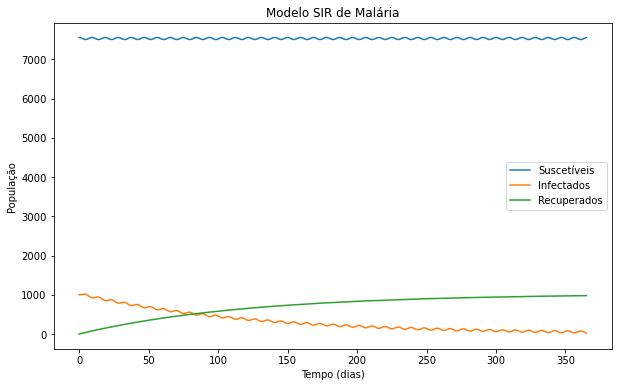
\includegraphics[width=1.25\linewidth]{SIR_Dados_Originais_Parham_Michael.png}
%   \captionof{figure}{A figure}
%   \label{fig:test1}
% \end{minipage}%
% \hspace{1.5cm} % Adiciona espaço horizontal
% \begin{minipage}{.45\textwidth}
%   \centering
%   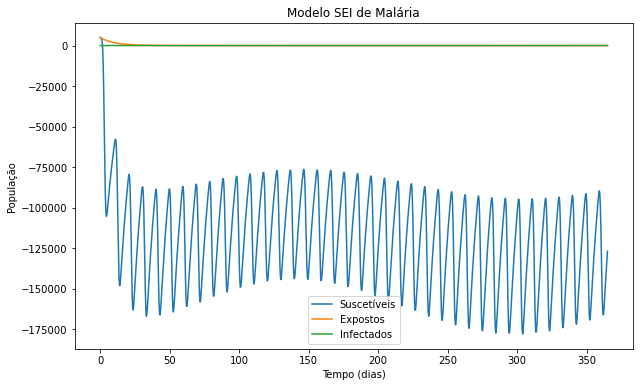
\includegraphics[width=1.3\linewidth]{SEI_Dados_Originais_Parham_Michael.png}
%   \captionof{figure}{Another figure} % Legenda à direita da segunda imagem
%   \label{fig:test2}
% \end{minipage}
% \end{figure}





\begin{figure}[!ht]
        \centering
        \hbox{\hspace{4em} 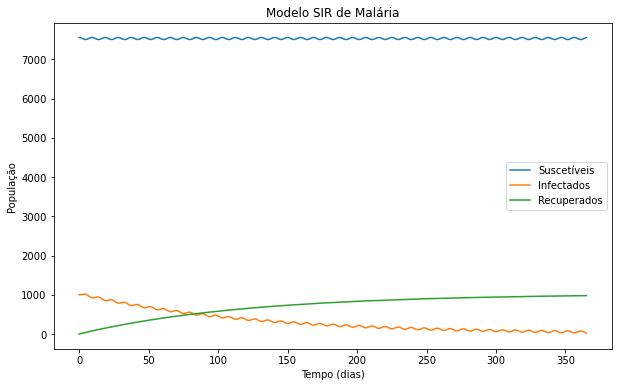
\includegraphics[scale=0.5] {SIR_Dados_Originais_Parham_Michael.png}}
        \caption{SIR com dados originais}
\end{figure} 
\begin{figure}[!ht]
        \centering
        \hbox{\hspace{3em} 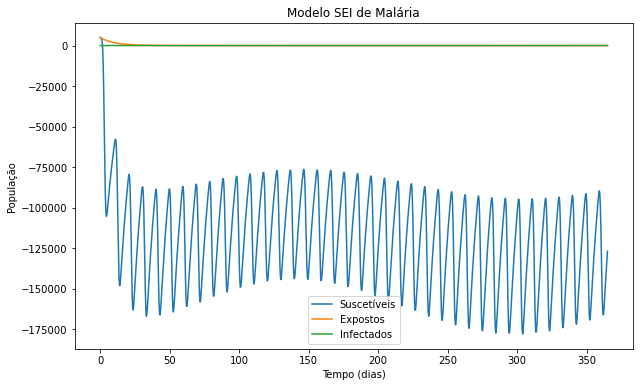
\includegraphics[scale=0.5] {SEI_Dados_Originais_Parham_Michael.png}}
        \caption{SEI com dados originais}
\end{figure} 
\newpage
Com essa modelagem inicial, é perceptível uma forte oscilação do número de humanos e mosquitos suscetíveis, assim como de humanos infectados. Ademais, é notável que, com esses parâmetros, a epidemia não irá se estabilizar, visto que o número de humanos infectados tende a 0 ao longo do ano, enquanto que a população de mosquitos suscetíveis fica negativa e a população de expostos e infectados também tende a 0. Esses efeitos foram caracterizados pela temperatura e precipitação oscilando em períodos de tempo muito curtos, devido a um alto valor de $\omega$ para ambas as funções. 
\\\\
Coletando dados climatológicos de Manaus em \cite{ClimaMANAUS}, a temperatura e precipitação média foram estimados como 26.4 $^\circ C$ e 250.083 mm, respectivamente. Com esses dados, a amplitude da variabilidade sazonal, frequência angular e ``phase lag" da variabilidade para ambos foram definidos de forma a aproximar os valores reais:
\\\\
\begin{adjustwidth}{-0.5cm}{}
\begin{center}
\renewcommand{\arraystretch}{1.5}
\begin{tabular}{|c | c|} 
 \hline
 \textbf{Parâmetro} & \textbf{Valor}\\ 
 \hline
  $T_1$ & \makecell[l]{\rule{0pt}{3ex}26.4$^\circ C$\rule[-1.5ex]{0pt}{0pt}} \\
 \hline
 $T_2$ & \makecell[l]{\rule{0pt}{3ex}0.025\rule[-1.5ex]{0pt}{0pt}} \\
 \hline
 $\omega_1$ & \makecell[l]{\rule{0pt}{3ex}0.017 (meses)$^{-1}$\rule[-1.5ex]{0pt}{0pt}} \\
 \hline
 $\phi_1$ & \makecell[l]{\rule{0pt}{3ex}-1.45\rule[-1.5ex]{0pt}{0pt}} \\
 \hline
 $R_1$ & \makecell[l]{\rule{0pt}{3ex}250.083 mm\rule[-1.5ex]{0pt}{0pt}} \\
 \hline
 $R_2$ & \makecell[l]{\rule{0pt}{3ex}0.565\rule[-1.5ex]{0pt}{0pt}} \\
 \hline
 $\omega_2$ & \makecell[l]{\rule{0pt}{3ex}0.02 (meses)$^{-1}$\rule[-1.5ex]{0pt}{0pt}} \\
 \hline
 $\phi_2$ & \makecell[l]{\rule{0pt}{3ex}1.6\rule[-1.5ex]{0pt}{0pt}} \\
 \hline
\end{tabular}
\captionof{table}{Valores dos parâmetros de clima}
\end{center}
\end{adjustwidth}

\vspace{1cm}
Os parâmetros de amplitude ($T_2$ e $R_2$) e defasagem de fase 
($\phi_1$ e $\phi_2$) são adimensionais. A temperatura e precipitação ao 
longo do ano evoluem então da seguinte maneira\footnote{A elaboração dos gráficos pode ser encontrada em
\\
https://github.com/RaphaLevy/TCC/blob/main/Discuss\%C3\%A3o/Correcao\_de\_Modelagens.ipynb}:


% \begin{figure}
% \hspace*{-1.5cm} % Adiciona espaço negativo para puxar a imagem para a esquerda
% \begin{minipage}{.45\textwidth}
%   \centering
%   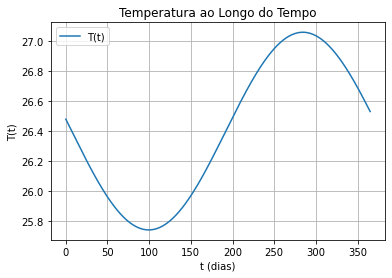
\includegraphics[width=1.2\linewidth]{Grafico_da_Temperatura.png}
%   \captionof{figure}{A figure}
%   \label{fig:test1}
% \end{minipage}%
% \hspace{1.5cm} % Adiciona espaço horizontal
% \begin{minipage}{.45\textwidth}
%   \centering
%   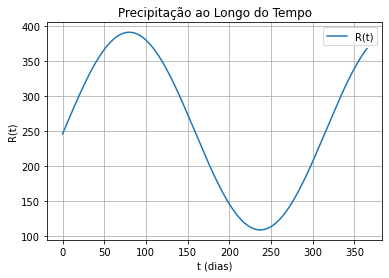
\includegraphics[width=1.2\linewidth]{Grafico_da_Precipitacao.png}
%   \captionof{figure}{Another figure} % Legenda à direita da segunda imagem
%   \label{fig:test2}
% \end{minipage}
% \end{figure}


\begin{figure}[!ht]
        \centering
        \hbox{\hspace{7.2em} 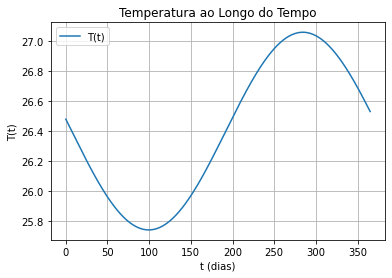
\includegraphics[scale=0.6] {Grafico_da_Temperatura.png}}
        \caption{Gráfico da temperatura}
\end{figure} 
\newpage
\begin{figure}[!ht]
        \centering
        \hbox{\hspace{7.5em} 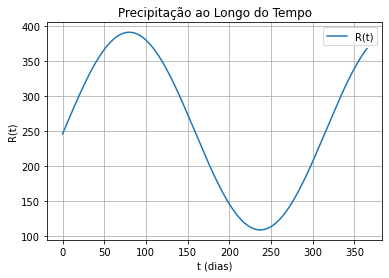
\includegraphics[scale=0.6] {Grafico_da_Precipitacao.png}}
        \caption{Gráfico da precipitação}
\end{figure} 
De forma a garantir a corretude da função com os parâmetros utilizados, calculei os valores da temperatura nos meses de outubro e maio, 
que são o mais quente e frio do ano, com temperaturas médias de 27.6 $^\circ C$ e 25.8 $^\circ C$ respectivamente, e da precipitação em 
março e agosto, que são os meses com maior e menor precipitação, com 395 e 114 mm, respectivamente. Os valores médios obtidos foram de 
27.06 $^\circ C$, 25.86 $^\circ C$, 390.67 mm e 112.89 mm. Tendo os parâmetros de $T$ e $R$ prontos para uma primeira análise, a evolução 
das populações de humanos e mosquitos foram verificadas utilizando $N=8558$, 
com $S_{H0} = 7558$, $I_{H0} = 10000$, $M= 300000$, $S_{M0}=250000$, $E_{M0} = 50000$, $A = 317.925, \ B = 15, \ C = -48.78$ e $R_L = 312 \ \text{mm}$. 
Os resultados podem ser encontrados no Apêndice 1 e 2 \footnote{A elaboração dos gráficos acima pode ser encontrada em
\\
https://github.com/RaphaLevy/TCC/blob/main/old/Testa\_Infectados\_Humanos.ipynb}. 
\\\\
Notavelmente, a modelagem resultante não está correta, com ambas as populações se tornando negativas em certos pontos, especialmente a da população humana, cujo número de infectados decai para aproximadamente -300000. Verificando as EDOs, foi possível ver que o único parâmetro que é dado em função da temperatura e chuva no SIR é o $a(T)$, que é a taxa de picadas por dia. Dada a sua fórmula, e sabendo que a temperatura inicialmente decai nos primeiros meses do ano, tem-se que $a$ tomará valores negativos na equação de infectados, visto que $T_1$ será maior que $T$ inicialmente, explicando o comportamento da curva. Se comparado com os dados do artigo de Parham e Michael, cuja temperatura é crescente inicialmente, foi necessário modificar a ordem do numerador dessa taxa para que, num primeiro momento, não se torne negativa conforme a temperatura decai. Utilizando então a equação $a(T) = \dfrac{T_1-T}{D_1}$, os resultados podem ser vistos no apêndice 3 e 4.
\\\\
Com essas modificações, a evolução da população humana parece mais viável do que estava anteriormente, com o número de infectados inicialmente baixo, 
aumentando ao longo do ano e posteriormente decaindo. Por outro lado, é possível notar que próximo do tempo final de análise, o número de humanos 
infectados se torna negativo. A modelagem de mosquitos, por sua vez, se manteve relativamente estável.
\\\\
Analisando o comportamento da modelagem de mosquitos de forma que a população ficasse aproximadamente constante ao longo do período, dadas as equações diferenciais do modelo SEI, e os parâmetros passados para atingir esse objetivo, o valor de $\mu$ passado fica muito próximo de 0, enquanto que $l(\tau_M)$, uma probabilidade, fica muito próxima de 1. Por isso, $\dfrac{dE_M}{dt}$ também fica bem próximo de 0, fazendo com que a função de expostos seja linear, aproximadamente constante no número inicial de infectados, enquanto que a população de mosquitos que sai do compartimento de suscetíveis quase que simultaneamente entra no compartimento de infectados, causando as ondulações espelhadas de $S$ e $I$. Para contornar esse efeito, foi necessário modificar o uso de $b_1$, para passar apenas mosquitos do compartimento $S$ para $E$, necessitando da inclusão de um novo parâmetro, $b_3$, para passar mosquitos do compartimento $E$ para $I$. Essa taxa é inversa ao período de incubação, então definimos
\begin{gather*}
    b_3 = \dfrac{T-T_{min}}{DD}
\end{gather*}
Ademais, foi removido o parâmetro $a(T)$ na passagem de mosquitos expostos para infectados, visto que nessa mudança do compartimento $E$ para $I$ não ocorrem novas picadas, assim como o parâmetro $T_1$ utilizado na fórmula de $a(T)$ também teve de ser modificado, visto que o artigo original aplica $T_1$ com dois valores diferentes, para a taxa de picadas e para a equação da temperatura por tempo. Com o intuito de manter a formatação de $T(t)$ e $R(t)$ a mesma, $T_1$ de $a$ foi modificado para $T'$.
\\\\
Considerando então o que foi dito acima, também se tornou necessário modificar as equações diferenciais do SEI, que ficaram dessa forma:
\begin{gather*}
\begin{cases}
\dfrac{dS_M}{dt} = b - ab_1\bigg(\dfrac{I_H}{N}\bigg)S_M - \mu S_M\\
\\
\dfrac{dE_M}{dt} = ab_1\bigg(\dfrac{I_H}{N}\bigg)S_M - \mu E_M - b_3E_Ml\\
\\
\dfrac{dI_M}{dt} = b_3E_Ml -\mu I_M\\
\end{cases}
\end{gather*}
\\\\
Com as adaptações feitas à transmissão da doença entre os mosquitos 
(Apêndices 5 e 6), é possível ver que não só o 
equilíbrio mudou, de forma que agora o número de 
expostos tende a 0, e não o de infectados, podemos ver também que a população 
de humanos é fortemente impactada, novamente oscilando constantemente, e com 
o número de infectados ficando negativo repetidas vezes \footnote{Observação: 
as modelagens do SIR mostradas ao longo de 5 anos de análise foram feitas 
usando o valor médio estimado para a população no período entre 2004 e 2008, 
com $N$=8558}.
Analisando modificações nos parâmetros empíricos citados acima, foi notado que esse comportamento se dá devido em especial ao alto valor em módulo de $A$, visto que com $A=-217.925$, o comportamento do modelo foi similar. Até mesmo usando $A=17.925$, o comportamento observado foi similar. Contudo, para $A=0$, a população humana teve um comportamento bem mais viável, enquanto que a população de mosquitos tendeu à extinção (Apêndices 7 e 8).
\footnote{A elaboração dos gráficos indicados acima pode ser encontrada em
\\
https://github.com/RaphaLevy/TCC/blob/main/Discuss\%C3\%A3o/Correcao\_de\_Modelagens\_2.ipynb}
\\\\
Analisando o efeito de $A$, notou-se que, para $A$ muito grande, $\mu$ se torna extremamente pequeno:
\begin{flalign*}
& \text{Para A} = 317.925, \ \mu = 4.505961269611858e-06 \\
& \text{Para A} = 17.925, \ \mu = 7.78802370175753e-05 \\
& \text{Para A} = -217.925, \ \mu = -6.599014101979344e-06 \\
& \text{Para A} = 0, \mu = 0.0028800184321179124
\end{flalign*}
Com isso, a mortalidade de mosquitos será extremamente baixa para valores 
grandes de $A$, positivos ou não. Contudo, como uma forma de possibilitar 
o uso de valores altos para esse parâmetro, e ainda garantir que as 
populações tenham valores sempre não-negativos, foi aplicado um máximo 
nas taxas com subtração, segundo recomendação do orientador, de forma que 
o valor resultante entre $T(t)-T_{min}$, $R_L - R(t)$ e $T'-T(t)$ seja o máximo entre essas diferenças e uma tolerância pequena, no caso 
foi utilizado um $\epsilon = 10^{-5}$. Isso foi suficiente para garantir que, 
mesmo com valores grandes de $A$, o modelo não tomasse valores 
negativos (Apêndices 9 a 12). 
\\\\
Com essas modificações, é possível notar como, independente do valor de $A$, a evolução das populações humanas será bem similar, com uma estabilização da população de suscetíveis logo antes de se tornar 0. A de mosquitos, por sua vez, é menos oscilante para valores grandes de $A$, e não se estabiliza mesmo em mais de 10000 dias. Por outro lado, se $A=0$, a população de mosquitos se aproxima da extinção, com pequenos picos de mosquitos unicamente suscetíveis, sem estabilização da doença. Contudo, ainda que usando o máximo entre um pequeno $\epsilon$ e as diferenças notadas acima, $T'=26.4$ é um valor menor que a temperatura máxima calculada para o ano, que é próxima de 27.1. Assim, foi recomendado pelo orientador que fosse testado um valor maior que esse máximo, no caso $T'=27.4$ (Apêndice 13 e 14).
\\\\
Tendo então o modelo SIR/SEI devidamente corrigido, foi possível partir para as análises de aplicação do desmatamento. Para isso, iniciei com o cálculo do $\mathcal{R}_0$ para ambos SIR e SEI, e também para o modelo acoplado, usando como referência a formulação de P. van den Driessche \cite{VANDENDRIESSCHE200229}:
\\\\
Definimos $X_s$ como o conjunto de todos os estados livres de doença, 
$$X_s=\{x \geq 0|x_i=0, i=1,\ldots,m\},$$
onde $X=(x_1,\ldots, x_n)^T$, tal que $x_i\geq 0$ seja o número de indivíduos em cada compartimento, e supomos cada função continuamente diferenciável pelo menos duas vezes em cada variável $(C^2)$.
\\\\
Agora, reordenamos as equações para que as $m$ primeiras sejam as que contém infectados. Seja ${\mathcal F}_i(x)$ a taxa de aparecimento de novas infecções no compartimento $i$, ${\mathcal V}_i^+(x)$ a taxa de entrada de indivíduos no compartimento $i$ por outros meios e ${\mathcal V}_i^-(x)$ a taxa de saída de indivíduos do compartimento $i$. O modelo de transmissão da doença consiste em condições iniciais não negativas juntamente com o seguinte sistema de equações:
$$\dot{x}=f_i(x)={\mathcal F}_i(x)-{\mathcal V}_i(x), i=1,\ldots, n,$$
em que ${\mathcal V}_i (x) = {\mathcal V}_i^{-}(x) - {\mathcal V}_i^+(x)$. Definimos também $F=\left[\frac{\partial {\mathcal F}_i (x_0)}{\partial x_j}\right]$ e $V=\left[\frac{\partial {\mathcal V}_i (x_0) }{\partial x_j}\right]$, onde $x_0$ é um DFE (Equilíbrio livre de doença) e $1\leq i,j \leq m$. 
\\\\
Isto equivale à jacobiana  destas duas matrizes, após substituir $x_0$ ou seja, $S=1$. $R_0$ será dado por $\rho(FV^{-1})$, ou seja, será o raio espectral da matriz $FV^{-1}$. Com as definições necessárias, podemos calcular o $R_0$ de ambos os modelos como a seguir:
\begin{itemize}
\item \textbf{SIR:}
Nesse caso, $m=1$, e nossos compartimentos serão colocados da forma $[I_H, S_H, R_H]$. Como o $R_0$ é calculado com valores normalizados, multiplicaremos as equações necessárias por $N$ para remover o denominador, e especificamente no caso do SIR, como $R_H$ não é utilizado em nenhuma das equações, podemos apenas fazer em função de $S$ e $I$. Portanto:
$$ {\mathcal F}_i(x): \text{ taxa de surgimento de novos infectados no compartimento } i $$
$$ {\mathcal F} =\begin{bmatrix}
a  b_2  I_M  S_H \\
\end{bmatrix} $$
Além disso, temos
$$ {\mathcal V}_i(x)^-: \text{ taxa de saída do compartimento } i $$
$$ {\mathcal V}_i(x)^+: \text{ taxa de entrada do compartimento } i $$
Logo:
$$
{\mathcal V^-} = \begin{bmatrix}
\gamma I_H\\
\end{bmatrix}
$$
$$
{\mathcal V^+} = \begin{bmatrix}
0\\
\end{bmatrix}
$$
$${\mathcal V}_i (x) = {\mathcal V}_i(x)^{-} - {\mathcal V}_i(x)^+$$
Então,
$$
{\mathcal V} =
\begin{bmatrix}
\gamma I_H\\
\end{bmatrix}
$$
\\
Portanto
$$ F = \dfrac{\partial{\mathcal F}}{\partial I_M} =\begin{bmatrix}
a  b_2  S_H \\
\end{bmatrix} $$
$$ V = \dfrac{\partial{\mathcal V}}{\partial I_H} =\begin{bmatrix}
\gamma \\
\end{bmatrix} $$
\\No equilíbrio, $[S_H^*, I_H^*] = [1,0]$, então $F=[a  b_2], \ V = [\gamma]$ e $R_0 = \Big | \dfrac{ab_2}{\gamma}\Big | $.

\item \textbf{SEI:}
Nesse caso, $m=2$, e nossos compartimentos serão colocados da forma $[E_M, I_M, S_M]$.Novamente multiplicaremos as equações necessárias por $N$ para remover o denominador. Portanto:
$$ {\mathcal F} =\begin{bmatrix}
a b_1 I_H S_M\\
0\\
\end{bmatrix} $$
$$
{\mathcal V^-} = \begin{bmatrix}
E_M (\mu + b_3 l)\\
\mu I_M
\end{bmatrix}
$$
$$
{\mathcal V^+} = \begin{bmatrix}
0\\
b_3 E_M l\\
\end{bmatrix}
$$
$${\mathcal V}_i (x) = {\mathcal V}_i(x)^{-} - {\mathcal V}_i(x)^+$$
Então,
$$
{\mathcal V} =
\begin{bmatrix}
E_M (\mu + b_3 l)\\
\mu I_M - b_3 E_M l\\
\end{bmatrix}
$$
\\
Portanto
$$ F = \dfrac{\partial{\mathcal F}}{\partial E_M, I_H} =\begin{bmatrix}
\dfrac{\partial ab_1 I_H S_M}{\partial E_M} & \dfrac{\partial ab_1 I_H S_M}{\partial I_H}\\
\dfrac{\partial 0}{\partial E_M} & \dfrac{\partial 0}{\partial I_H}\\
\end{bmatrix} = 
\begin{bmatrix}
0 & ab_1 S_M\\
0 & 0\\
\end{bmatrix}$$
$$ V = \dfrac{\partial{\mathcal V}}{\partial E_M, I_M} =\begin{bmatrix}
\dfrac{\partial E_M (\mu + b_3 l)}{\partial E_M} & \dfrac{\partial E_M (\mu + b_3 l)}{\partial I_M}\\
\dfrac{\partial \mu I_M - b_3 E_M l}{\partial E_M} & \dfrac{\partial \mu I_M - b_3 E_M l}{\partial I_M}\\
\end{bmatrix} = 
\begin{bmatrix}
\mu+b_3 l & 0\\
- b_3 l & \mu\\
\end{bmatrix}$$
\\No equilíbrio, $[S_M^*, E_M^*, I_M^*] = [1,0,0]$, então $$F=\begin{bmatrix}
0 & ab_1\\
0 & 0\\
\end{bmatrix},$$
$$V = \begin{bmatrix}
\mu+b_3 l & 0\\
- b_3 l & \mu\\
\end{bmatrix}$$ e $R_0 = \Big | \dfrac{ab_1b_3l}{(b_3l+\mu)\mu}\Big | $.

\item \textbf{SIR/SEI:}
Nesse caso, $m=3$, e nossos compartimentos serão colocados da forma $[I_H, E_M, I_M, S_H, S_M]$.Novamente multiplicaremos as equações necessárias por $N$ para remover o denominador. Portanto:
$$ {\mathcal F} =\begin{bmatrix}
a  b_2  I_M  S_H \\
a b_1 I_H S_M\\
0\\
\end{bmatrix} $$
$$
{\mathcal V^-} = \begin{bmatrix}
\gamma I_H\\
E_M (\mu + b_3 l)\\
\mu I_M
\end{bmatrix}
$$
$$
{\mathcal V^+} = \begin{bmatrix}
0\\
0\\
b_3 E_M l\\
\end{bmatrix}
$$
$${\mathcal V}_i (x) = {\mathcal V}_i(x)^{-} - {\mathcal V}_i(x)^+$$
Então,
$$
{\mathcal V} =
\begin{bmatrix}
I_H \gamma \\
E_M (\mu + b_3 l)\\
\mu I_M - b_3 E_M l\\
\end{bmatrix}
$$
\\
Portanto
$$ F = \dfrac{\partial{\mathcal F}}{\partial I_H, E_M, I_M} =\begin{bmatrix}
\dfrac{\partial ab_2 I_M S_H}{\partial I_H} & \dfrac{\partial ab_2 I_M S_H}{\partial E_M} & \dfrac{\partial ab_2 I_M S_H}{\partial I_M}\\
\dfrac{\partial ab_1 I_H S_M}{\partial I_H} & \dfrac{\partial ab_1 I_H S_M}{\partial E_M} & \dfrac{\partial ab_1 I_H S_M}{\partial I_M}\\
\dfrac{\partial 0}{\partial I_H} & \dfrac{\partial 0}{\partial E_M} & \dfrac{\partial 0}{\partial I_M}\\
\end{bmatrix} = 
\begin{bmatrix}
0 & 0 & ab_2 S_H\\
ab_1 S_M & 0 & 0\\
0 & 0 & 0
\end{bmatrix}$$
$$ V = \dfrac{\partial{\mathcal V}}{\partial I_H, E_M, I_M} =\begin{bmatrix}
\dfrac{\partial \gamma I_H}{\partial I_H} & \dfrac{\partial \gamma I_H}{\partial E_M} & \dfrac{\partial \gamma I_H}{\partial I_M}\\
\dfrac{\partial E_M (\mu + b_3 l)}{\partial I_H} & \dfrac{\partial E_M (\mu + b_3 l)}{\partial E_M} & \dfrac{\partial E_M (\mu + b_3 l)}{\partial I_M}\\
\dfrac{\partial \mu I_M - b_3 E_M l}{\partial I_H} & \dfrac{\partial \mu I_M - b_3 E_M l}{\partial E_M} & \dfrac{\partial \mu I_M - b_3 E_M l}{\partial I_M}\\
\end{bmatrix} = 
\begin{bmatrix}
\gamma & 0 & 0\\
0 & b_3l+\mu & 0\\
0 & -b_3l & \mu
\end{bmatrix}$$
\\No equilíbrio, $[S_H^*, S_M^*, I_H^*, E_M^*, I_M^*] = [1,1,0,0,0]$, então $$F=\begin{bmatrix}
0 & 0 & ab_2\\
ab_1 & 0 & 0\\
0 & 0 & 0
\end{bmatrix},$$
$$V = \begin{bmatrix}
\gamma & 0 & 0\\
0 & b_3l+\mu & 0\\
0 & -b_3l & \mu
\end{bmatrix}$$ 
e $R_0 = \Big | \sqrt{\dfrac{a^2 b_1 b_2 b_3 l}{(b_3 l + \mu)\gamma \mu}}\Big | = 
\sqrt{\mathcal{R}_{0 SIR} \times \mathcal{R}_{0 SEI}}$. 

\end{itemize}
Tendo obtido a fórmula fechada de $\mathcal{R}_0$, foi possível calcular o seu valor para o 
modelo atual, apresentado nos apêndices 13 e 14. No caso, $\mathcal{R}_0$ = 88.16804666190774
e a taxa de picadas no tempo $t=0$ foi de 0.025218306088151666, ou seja, aproximadamente 
uma picada por mosquito a cada 40 dias. Notavelmente, esses são valores muito altos para 
o número de reprodução de uma doença, nesse caso indicando que um indíviduo poderia infectar 
outros 88. Sendo assim, seria necessário modificar os parâmetros para que o valor de 
$\mathcal{R}_0$ ficasse próximo de 1, para que seja mais fácil analisar como pequenas 
modificações nos parâmetros causariam a extinção ou a continuação da doença. 
Antes disso, porém, 
foi necessário mais uma vez corrigir as equações do SEI, já que a probabilidade diária de 
sobrevivência de mosquitos durante o ciclo de esporozoitos ($l$), não é diretamente associada 
à taxa de infecção dos expostos, e também não é parte da taxa de entrada de novos indíviduos 
no compartimento $I$. Outra coisa que teve de ser corrigida foi a fórmula da taxa de picadas 
($a$), que voltou a ser $\dfrac{(T(t) - T')}{D_1}$ como originalmente. As equações corrigidas 
do SEI ficaram como a seguir:
\begin{gather*}
\begin{cases}
\dfrac{dS_M}{dt} = b - ab_1\bigg(\dfrac{I_H}{N}\bigg)S_M - \mu S_M\\
\\
\dfrac{dE_M}{dt} = ab_1\bigg(\dfrac{I_H}{N}\bigg)S_M - \mu E_M - b_3E_M -lE_M\\
\\
\dfrac{dI_M}{dt} = b_3E_M -\mu I_M\\
\end{cases}
\end{gather*}
Tendo corrigido as equações, o $\mathcal{R}_0$ do SEI e do modelo acoplado foram $\Big | \dfrac{ab_1b_3}{(b_3+l+\mu)\mu}\Big | $ e $\Big | \sqrt{\dfrac{a^2b_1b_2b_3}{(b_3+l+\mu)\gamma\mu}}\Big | $, respectivamente. Podemos verificar que $\mathcal{R}_0$ é de fato adimensional: $a, \ b_3, \ l, \ \mu$ e $\gamma$ são funções de unidade 1/dia, enquanto $b_1$ e $b_2$ são adimensionais. Sendo assim, $\mathcal{R}_0$ do SIR tem dimensão (1/dia)/(1/dia), $\mathcal{R}_0$ do SEI tem dimensão (1/dia$^2$)/(1/dia$^2$) e o acoplado tem dimensão (1/dia$^3$)/(1/dia$^3$). 
\\\\
Novamente calculando o $\mathcal{R}_0$ do modelo atual, seu valor para o modelo acoplado 
foi de 63.745319442750855, o que já é menor que o encontrado previamente, mas ainda muito alto. 
Foi necessário analisar que parâmetros poderiam ser modificados de forma que $\mathcal{R}_0$ 
se aproximasse de 1 tanto para o SIR quanto para o SEI, já que pelas equações é possível 
aproximar o valor acoplado de 1 enquanto que o valor de um dos outros dois modelos fosse 
menor que 1, fazendo com que a doença não se estabilizasse ou a população tendesse à extinção, 
no caso do SEI.
\\
Dessa maneira, as modificações ideais para aproximar $\mathcal{R}_0$ de 1 foram as seguintes:
\begin{flalign*}
& T' = 27.4 \Rightarrow 25.6 \\
& D_1 = 36.5 \Rightarrow 55 \\
& A = 317.925 \Rightarrow 15 \\
& b_2 = 0.3 \Rightarrow 0.2 \\
& \gamma = 1/1825 \Rightarrow 1/365
\end{flalign*}
Com essas adaptações, 
\begin{flalign*}
& \mathcal{R}_0 \ \text{SIR} = 1.167378607783994 \\
& \mathcal{R}_0 \ \text{SEI} = 1.7805860145371295 \\
& \mathcal{R}_0 \ \text{SIR/SEI} = 1.4417413161486372
\end{flalign*}
\begin{figure}[!ht]
        \centering
        \hbox{\hspace{3.5em} 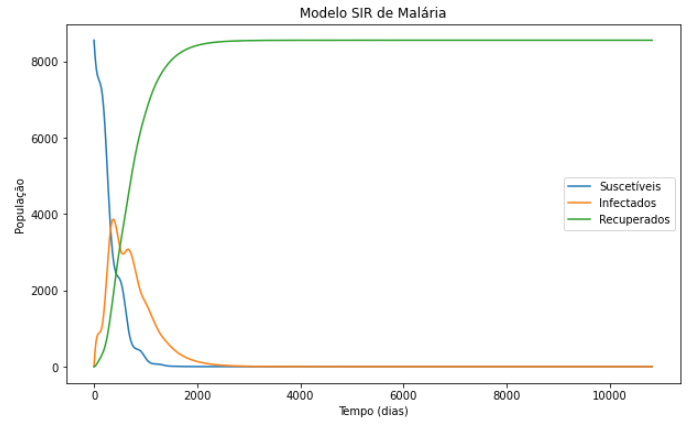
\includegraphics[scale=0.6] {SIR_R0_near1.png}}
        \caption{SIR com $T'=25.6 ^\circ C, \ A=15 \ (^\circ C^2 \ \text{dias})^{-1}, \ D_1=55 \ (^\circ C \ \text{dias}), \ b_2=0.2, \ \gamma=1/365$}
\end{figure} 
\begin{figure}[!ht]
        \centering
        \hbox{\hspace{3.5em} 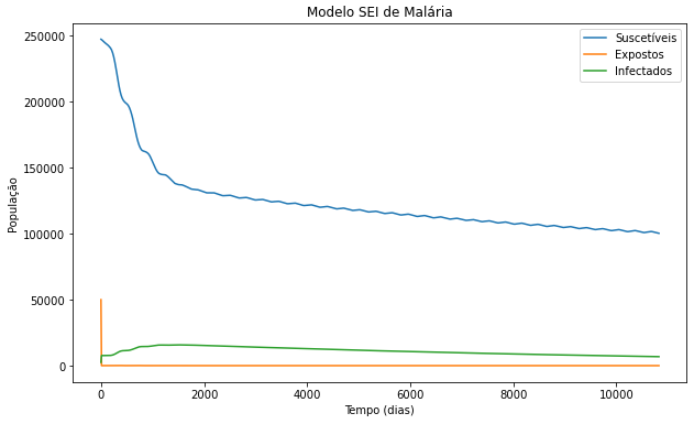
\includegraphics[scale=0.6] {SEI_R0_near1.png}}
        \caption{SEI com $T'=25.6 ^\circ C, \ A=15 \ (^\circ C^2 \ \text{dias})^{-1}, \ D_1=55 \ (^\circ C \ \text{dias}), \ b_2=0.2, \ \gamma=1/365$}
\end{figure}
\\\\
Discutindo essa aproximação de $\mathcal{R}_0$ a 1 com o orientador do 
Trabalho, foi decidido 
que ao invés de aumentar o valor $D_1$, um parâmetro empírico usado para 
estabilizar a taxa de picadas, seria ideal modificar $b_1$ e $b_2$, que são as
proporções de picadas gerando infecção em mosquitos e humanos suscetíveis, 
respectivamente, tendo em vista que, conforme temos mais ocorrências de áreas 
desmatadas, haverá um maior contato entre humanos e mosquitos, aumentando a 
proporção de picadas gerando infecção. 
\\\\
Junto com essa correção, também 
foram modelados os gráficos de evolução das taxas utilizadas, em função 
da temperatura e precipitação, ao invés do tempo, para que fosse 
possível analisar o comportamento dessas taxas conforme a temperatura e 
precipitação variam. Os gráficos estão indicados no apêndice, partindo do 15. 
Gerando esses gráficos, também foi percebido que seria ideal aumentar $R_L$ 
do valor atual de 312 mm para 450 mm, para evitar que a probabilidade de 
sobrevivência de mosquitos durante as diferentes fases se 
tornasse muito próximo de 0, o que estava afetando a taxa de 
nascimentos $b(R,T)$, e diminuir $\gamma$ de 1/365 dias para 1/120, valor original
do artigo de referência \cite{Parham2010}, de forma que a curva epidêmica fosse mais
próxima do analisado na realidade, visto na Figura 5 que a curva de infectados começa
a crescer logo no início da análise, e a infecção só deixa de ocorrer após mais de
5 anos.
\\\\
Após o desenvolvimento dos gráficos das taxas, foi iniciada a modelagem usando os dados 
``reais" da população obtidos através da interpolação dos dados de população de Manaus indicada na Tabela 4.
Com os valores previmente obtidos, a taxa anual de nascimentos foi estimada como sendo de 206.8 
nascimentos por ano. Sendo assim, são 0.56657 nascimentos por dia, aproximadamente, e 0.00007 nascimentos
diários por pessoa, já que a população rural média em Manaus é de aproximadamente 8078.5 pessoas entre 2004 e 2008.
\\\\
Assumindo que a taxa de natalidade e mortalidade de humanos é a mesma, foi então incluído na 
modelagem o parâmetro $\mu_H$, com valor 0.00007, representando a taxa diária de 
nascimentos e mortes. O modelo atualizado ficou como a seguir:
\begin{gather*}
\begin{cases}
\dfrac{dS_H}{dt} = \mu_HN-ab_2\bigg(\dfrac{I_M}{N}\bigg)S_H - \mu_HS_H\\
\\
\dfrac{dI_H}{dt} = ab_2\bigg(\dfrac{I_M}{N}\bigg)S_H-\gamma I_H - \mu_HI_H\\
\\
\dfrac{dR_H}{dt} = \gamma I_H - \mu_HR_H\\
\\
\end{cases}
\end{gather*}
A elaboração dos gráficos, a partir do Apêndice 27, foi feita em \footnote{https://github.com/RaphaLevy/TCC/blob/main/Modelagem\_com\_Dinamica\_Pop/ \\
Modelagem\_com\_Entrada\_Populacional.ipynb}.
\\\\
Tendo corrigido as equações, o $\mathcal{R}_0$ do SIR e do modelo acoplado 
foram $\Big | \dfrac{ab_2}{\gamma + \mu_H}\Big | $ e 
$\Big | \sqrt{\dfrac{a^2b_1b_2b_3}{(b_3+l+\mu)(\gamma+\mu_H)\mu}}\Big | $, respectivamente. Podemos verificar que $\mathcal{R}_0$ é de fato adimensional: $a, \ b_3, \ l, \ \mu$ e $\gamma$ são funções de unidade 1/dia, enquanto $b_1$ e $b_2$ são adimensionais. Sendo assim, $\mathcal{R}_0$ do SIR tem dimensão (1/dia)/(1/dia), $\mathcal{R}_0$ do SEI tem dimensão (1/dia$^2$)/(1/dia$^2$) e o acoplado tem dimensão (1/dia$^3$)/(1/dia$^3$). 
\\\
Como esperado, com $\mathcal{R}_0$ menor que 1, e apenas 1 mosquito exposto e 
1 humano infectado, a doença não consegue se estabelecer, como pode ser visto abaixo:
\begin{figure}[!ht]
        \centering
        \hbox{\hspace{2.5em} 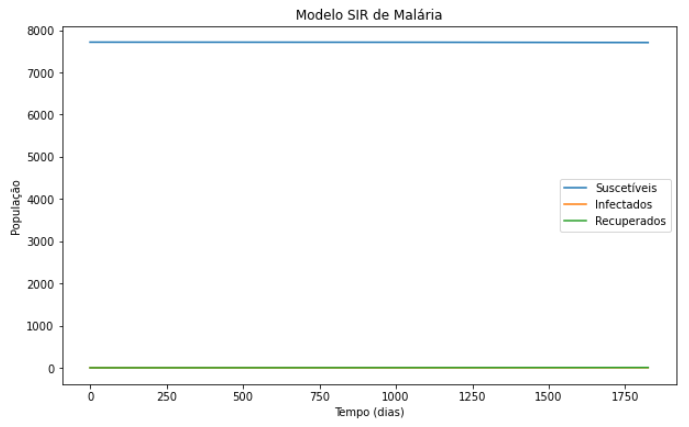
\includegraphics[scale=0.7] {SIR_Entrada_Pop_1_1_Infect.png}}
        \caption{SIR com $T'=25.6 ^\circ C, \ A=12.5 \ (^\circ C^2 \ \text{dias})^{-1}, \ B=15 \ (^\circ C \ \text{dias})^{-1}, \ C=-48.78 \ (\text{dias})^{-1}, \ R_L=450 \text{mm}, E_{M0}=1, I_{H0}=1$} 
\end{figure} 
\begin{figure}[!ht]
        \centering
        \hbox{\hspace{2.5em} 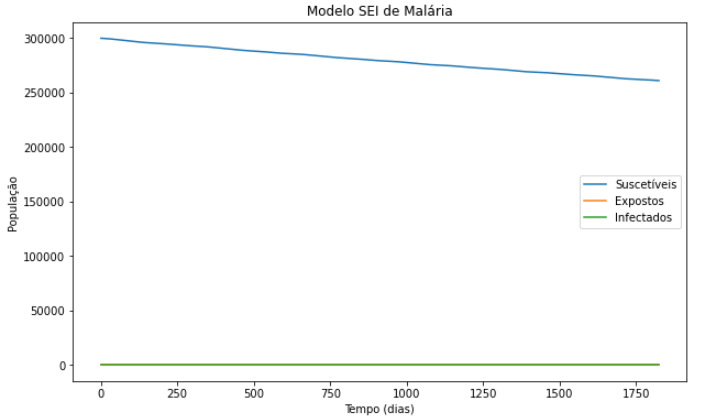
\includegraphics[scale=0.7] {SEI_Entrada_Pop_1_1_Infect.png}}
        \caption{SEI com $T'=25.6 ^\circ C, \ A=12.5 \ (^\circ C^2 \ \text{dias})^{-1}, \ B=15 \ (^\circ C \ \text{dias})^{-1}, \ C=-48.78 \ (\text{dias})^{-1}, \ R_L=450 \text{mm}, E_{M0}=1, I_{H0}=1$} 
\end{figure} 
\\Dos apêndices 27 a 30, aumentando o número de infectados e expostos, inicialmente com um 
``pequeno" aumento, com 1/30 da população de mosquitos exposta à doença, e 6.5\% 
de humanos infectados, a população de infectados humanos começa a aumentar, 
mas não consegue se estabelecer. Prolongando o tempo de análise, será possível 
ver que a população se extinguirá nos anos seguintes. Idealmente, seria 
possível verificar a população de infectados tendendo a 0 ainda no tempo da 
análise. Por outro lado, iniciando a população humana com cerca de 13\% de infectados, 
é possível ver que essa população tem um aumento ao longo do primeiro ano, 
chegando a quase 41\% da população, mas posteriormente decaindo.
\\\\
No caso dos mosquitos, a população inicial de expostos quase que 
imediatamente se torna de infectados, se estabilizando em cerca de 5000 
indivíduos, mas não é possível perceber a população de infectados se 
extinguindo, mesmo prolongando o tempo de análise. Esse comportamento 
ainda pode ser notado quando 1/3 da população começa exposto, rapidamente 
se tornando infectada, mas se estabelecendo em cerca de 10000 indivíduos. 
\\\\
Agora, voltando a um único exposto e infectado inicialmente, e incluindo um fator
multiplicativo $k$ nas proporções $b_1$ e $b_2$, representando o aumento de contato
entre humanos e mosquitos devido ao desmatamento, foi possível analisar o efeito desse impacto
na evolução da doença. A formulação final do modelo ficou como a seguir:
\begin{gather*}
\begin{cases}
\dfrac{dS_H}{dt} = \mu_HN-akb_2\bigg(\dfrac{I_M}{N}\bigg)S_H - \mu_HS_H\\
\\
\dfrac{dI_H}{dt} = akb_2\bigg(\dfrac{I_M}{N}\bigg)S_H-\gamma I_H - \mu_HI_H\\
\\
\dfrac{dR_H}{dt} = \gamma I_H - \mu_HR_H\\
\\
\dfrac{dS_M}{dt} = b - akb_1\bigg(\dfrac{I_H}{N}\bigg)S_M - \mu S_M\\
\\
\dfrac{dE_M}{dt} = akb_1\bigg(\dfrac{I_H}{N}\bigg)S_M - \mu E_M - b_3E_M -lE_M\\
\\
\dfrac{dI_M}{dt} = b_3E_M -\mu I_M\\
\end{cases}
\end{gather*}
Aumentando as proporções em 20 e 50\% ($k=1.2$ e $k=1.5$), não foi possível perceber
nenhuma diferença visível na evolução da doença, isso porque $\mathcal{R}_0 < 1$  
para $k < 2.0746963059512207$, como pode ser visto abaixo:
\begin{figure}[!ht]
        \centering
        \hbox{\hspace{3em} 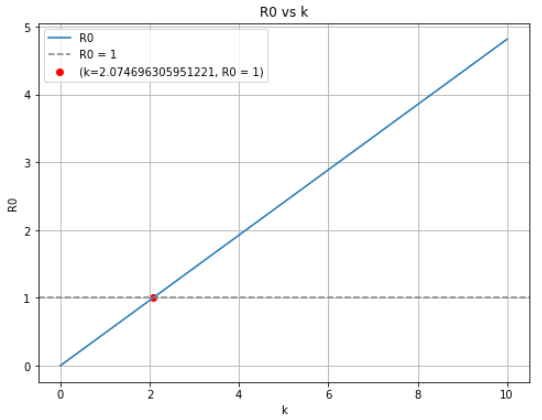
\includegraphics[scale=0.8] {Plot_R0_vs_k.png}}
        \caption{$\mathcal{R}_0$ em função de $k$}
\end{figure} 
\\\\
%mas com um aumento de 100\%, o resultado ficou como a seguir:
Sendo assim, mesmo um aumento de 100\% nas proporções de picadas causando infecção
não seria suficiente para que a doença se torne endêmica. Abaixo estão testes com $k=2.5, \ 5$ e $10$:
\begin{figure}[!ht]
        \centering
        \hbox{\hspace{2.0em} 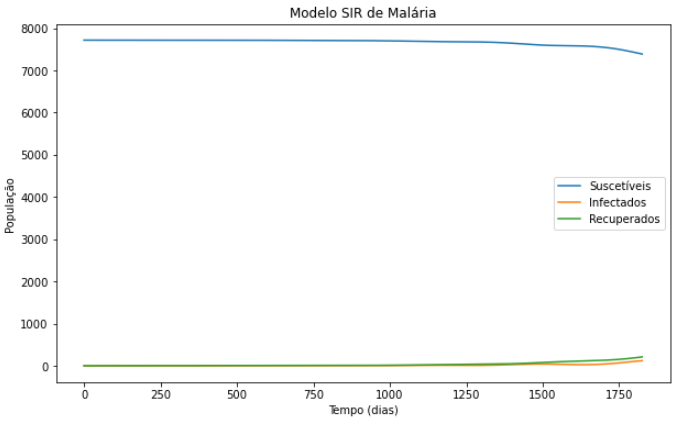
\includegraphics[scale=0.7] {Correcao_SIR_Desmat_k=2_5.png}}
        \caption{SIR com $T'=25.6 ^\circ C, \ A=12.5 \ (^\circ C^2 \ \text{dias})^{-1}, \ B=15 \ (^\circ C \ \text{dias})^{-1}, \ C=-48.78 \ (\text{dias})^{-1}, \ R_L=450 \text{mm}, \ k=2.5$}
\end{figure} 
\begin{figure}[!ht]
        \centering
        \hbox{\hspace{1.5em} 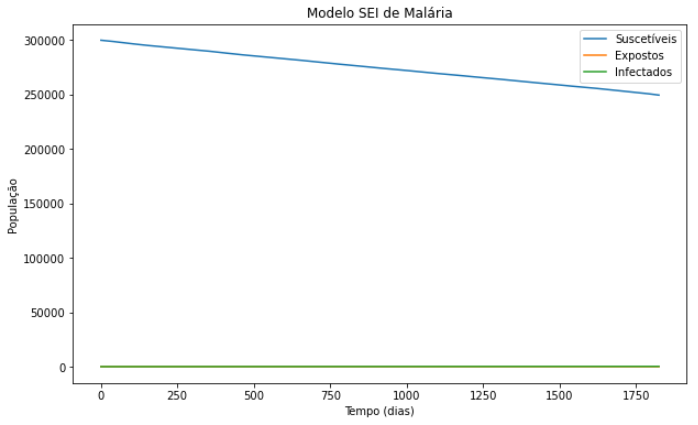
\includegraphics[scale=0.7] {Correcao_SEI_Desmat_k=2_5.png}}
        \caption{SEI com $T'=25.6 ^\circ C, \ A=12.5 \ (^\circ C^2 \ \text{dias})^{-1}, \ B=15 \ (^\circ C \ \text{dias})^{-1}, \ C=-48.78 \ (\text{dias})^{-1}, \ R_L=450 \text{mm}, \ k=2.5$}
\end{figure} 
\newpage
Aumentando em $150\%$ a proporção de picadas causando infecção, já é possível notar que o 
número de infectados começa a aumentar, ainda que quase no final do período 
de análise. Isso porque com o aumento em $k$, $\mathcal{R}_0$ passou de 0.48, 
com $k=1$, para 1.2, permitindo que a doença se estabeleça a longo prazo. Como $k$
está relacionado tanto com $b_1$ quanto $b_2$, esse fator aparecerá como $k^2$ no
numerador de $\mathcal{R}_0$, portanto afetando seu valor de forma linear.
Aumentando $k$ para 5, será bem mais perceptível a evolução da doença:
\begin{figure}[!ht]
        \centering
        \hbox{\hspace{3.7em} 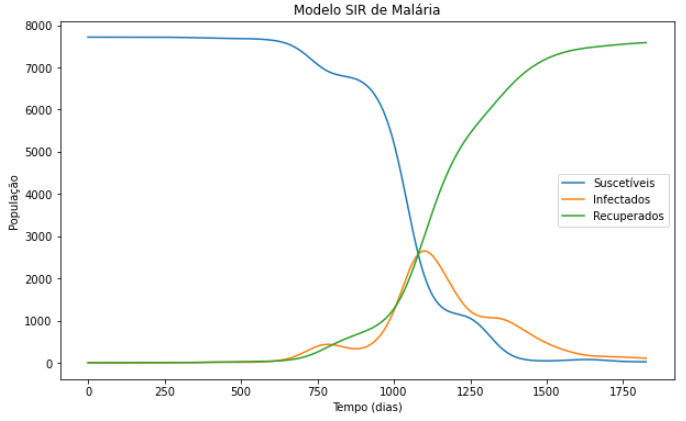
\includegraphics[scale=0.6] {Correcao_SIR_Desmat_k=5.png}}
        \caption{SIR com $T'=25.6 ^\circ C, \ A=12.5 \ (^\circ C^2 \ \text{dias})^{-1}, \ B=15 \ (^\circ C \ \text{dias})^{-1}, \ C=-48.78 \ (\text{dias})^{-1}, \ R_L=450 \text{mm}, \ k=5$}
\end{figure} 
\begin{figure}[!ht]
        \centering
        \hbox{\hspace{3.2em} 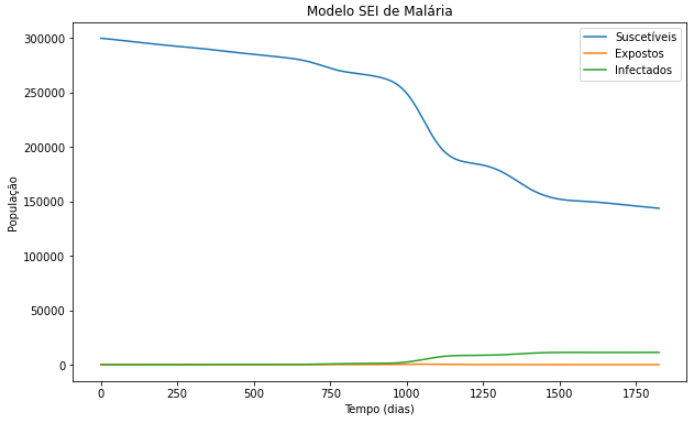
\includegraphics[scale=0.6] {Correcao_SEI_Desmat_k=5.png}}
        \caption{SEI com $T'=25.6 ^\circ C, \ A=12.5 \ (^\circ C^2 \ \text{dias})^{-1}, \ B=15 \ (^\circ C \ \text{dias})^{-1}, \ C=-48.78 \ (\text{dias})^{-1}, \ R_L=450 \text{mm}, \ k=5$}
\end{figure} 
\newpage
Nesse caso, $\mathcal{R}_0 = 2.41$, e apesar de não ser possível verificar no tempo 
máximo dos 5 anos, nesse caso o número de infectados consegue se estabilizar, 
oscilando em aproximadamente 50 humanos e 9000 mosquitos infectados. Aumentando $k$ para 10, 
$\mathcal{R}_0 = 4.82$, e a infecção atinge seu máximo de forma ainda mais rápida:
\begin{figure}[!ht]
        \centering
        \hbox{\hspace{4.2em} 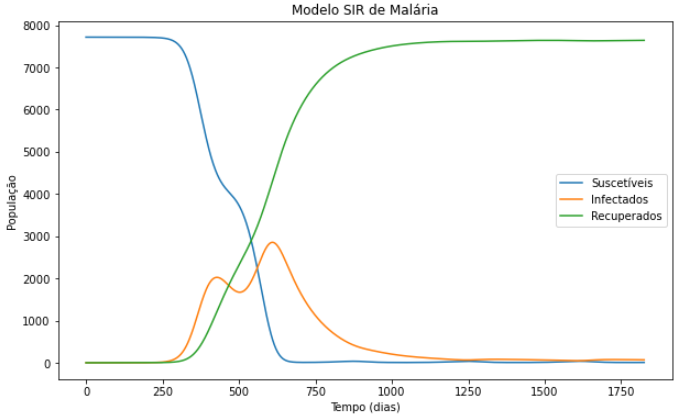
\includegraphics[scale=0.6] {Correcao_SIR_Desmat_k=10.png}}
        \caption{SIR com $T'=25.6 ^\circ C, \ A=12.5 \ (^\circ C^2 \ \text{dias})^{-1}, \ B=15 \ (^\circ C \ \text{dias})^{-1}, \ C=-48.78 \ (\text{dias})^{-1}, \ R_L=450 \text{mm}, \ k=10$}
\end{figure} 
\begin{figure}[!ht]
        \centering
        \hbox{\hspace{4.2em} 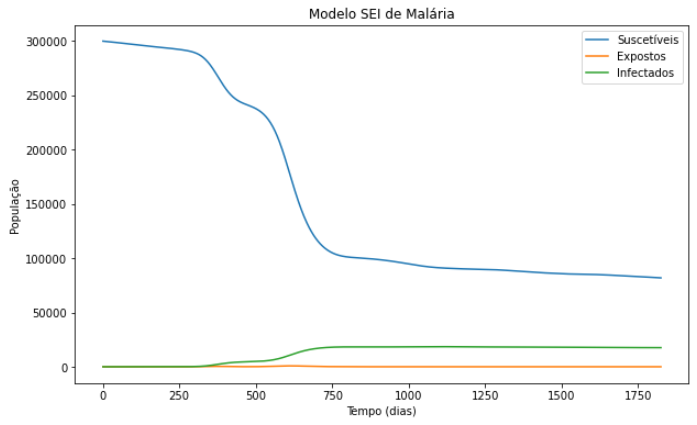
\includegraphics[scale=0.6] {Correcao_SEI_Desmat_k=10.png}}
        \caption{SEI com $T'=25.6 ^\circ C, \ A=12.5 \ (^\circ C^2 \ \text{dias})^{-1}, \ B=15 \ (^\circ C \ \text{dias})^{-1}, \ C=-48.78 \ (\text{dias})^{-1}, \ R_L=450 \text{mm}, \ k=10$}
\end{figure} 
\newpage
Com esses resultados, é possível perceber que o desmatamento acarretando em aproximação
entre hospedeiro e vetor causa um alto impacto na dinâmica da malária,
dado que mesmo com um único indivíduo infectado, a doença se estabelece e atinge 
um nível de infecção humana de cerca de $40\%$ da população conforme a 
proporção de picadas causando infecção aumenta. Agora, podemos encontrar qual é o valor de $I_H$
no equilíbrio dependendo de $k$:
\begin{figure}[!ht]
        \centering
        \hbox{\hspace{4.2em} 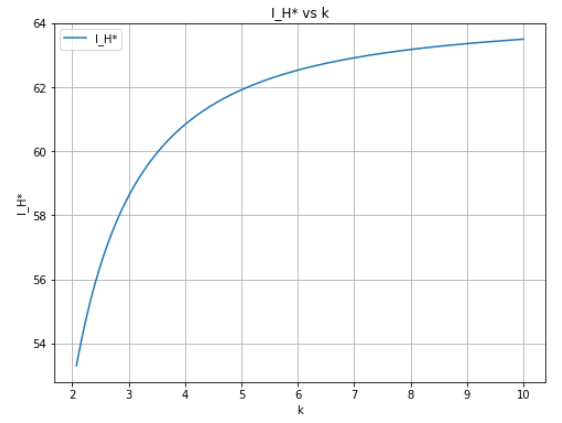
\includegraphics[scale=0.7] {Plot_I_H_vs_k.png}}
        \caption{$I_H^*$ em função de $k$}
\end{figure} 
\\\\
Iniciando o plot a partir de $k$ que deixa $\mathcal{R}_0 = 1$, é possível ver que
o equilíbrio endêmico da população humana se aproxima de 64 conforme $k$ se aproxima de 10.
Mais especificamente, quando $k=10$, $I_H^* \approx 63.49$ \footnote{A elaboração 
dos gráficos em função de $k$ podem ser encontrados em https://github.com/RaphaLevy/TCC/blob/main/Modelagem\_com\_Dinamica\_Pop/Plota\_Equilibrio\_e\_R0.ipynb. 
O cálculo dos equilíbrios pode ser encontrado em
https://github.com/RaphaLevy/TCC/blob/main/Modelagem\_com\_Dinamica\_Pop/R0\_com\_Dinamicas\_Demograficas.ipynb}.
Analisando o equilíbrio de suscetíveis conforme $k$ aumenta, é possível 
ver o equilíbrio decaindo rapidamente
de $N$ quando $k=0$ para aproximadamente 5000 indivíduos quando $k=1$. Analisando 
nos valores de $k$ tais que $\mathcal{R}_0 \geq 1$:
\begin{figure}[!ht]
        \centering
        \hbox{\hspace{4.2em} 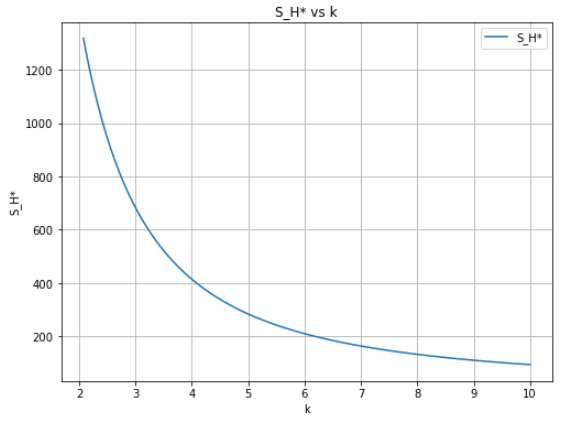
\includegraphics[scale=0.7] {Plot_S_H_vs_k.png}}
        \caption{$S_H^*$ em função de $k$}
\end{figure} 
\newpage
Nesse caso, a população de suscetíveis tende a aproximadamente 95 conforme 
$k$ se aproxima de 10. Tendo calculado os equilíbrios de $S_H$ e $I_H$,
foi possível fazer uma análise de estabilidade global. Como estamos interessados
em analisar o equilíbrio endêmico, utilizei $k=10$:
\begin{figure}[!ht]
        \centering
        \hbox{\hspace{2.2em} 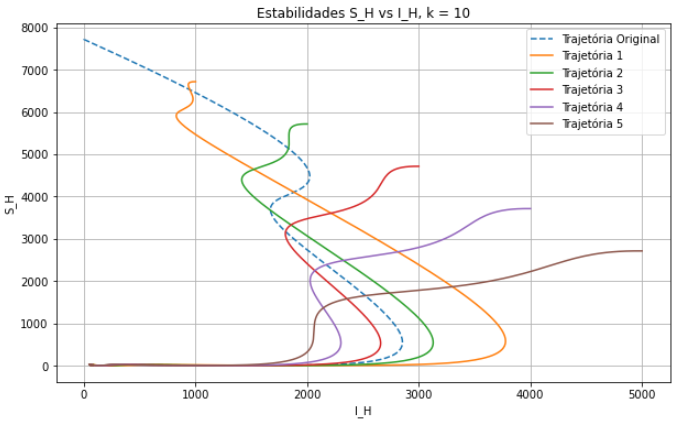
\includegraphics[scale=0.7] {Equilibrio_SH_IH_k_10.png}}
        \caption{Equilíbrio global $S_H^* \times I_H^*$ para $k=10$}
\end{figure}
\\\\
Nesse caso, foram feitas 6 análises, a primeira utilizando os
valores iniciais de $S_H$ e $I_H$ como sendo 7716 e 1, e as demais aumentando $I_H$ 
em 1000 e diminuindo $S_H$ em 1000 indivíduos. Nesse caso, é possível
ver as populações de suscetíveis e infectados com um equilíbrio final de
aproximadamente 8 e 70 pessoas, respectivamente. Com isso,
poderíamos comparar o resultado obtido com o cálculo do equilíbrio endêmico de Adda e Bichara
\cite{adda2011global}, onde
\begin{gather*}
        S_H^* = \dfrac{1}{\mathcal{R}_0} \\
        I_H^* = \dfrac{\mu_H}{\mu_H+\gamma}(1-\dfrac{1}{\mathcal{R}_0})
\end{gather*}       
Através desse cálculo, a população de suscetíveis e infectados no equilíbrio 
foi de aproximadamente 1601 e 51, respectivamente. Notavelmente, esses valores 
estão destoantes dos 
obtidos através do cálculo numérico. Contudo, é necessário considerar a principal diferença entre as equações
propostas para $S$ e $I$ nesse Trabalho e no artigo de Adda e Bichara, que é o uso de
$I_M$ na taxa de infecção $\beta$, dada a dinâmica do modelo 
acoplado de SIR e SEI nesse caso, que não está sendo considerada no trabalho
de Adda e Bichara.

\chapter{Discussão}

Ao longo do trabalho, foi desenvolvido e analisado um modelo de transmissão 
SIR/SEI para a malária de forma a complementar a metodologia original de Parham \& Michael, 
utilizando dos fatores epidemiológicos da transmissão da doença e complementando com 
dinâmicas de demografia humana e fatores ambientais externos à temperatura e precipitação,
como o desmatamento, considerado no fator multiplicativo das proporções de picadas
causando infecção. 
\\\\
Dado o grande foco alocado na modelagem da transmissão analisando os impactos 
ambientais, sendo necessárias diferentes adaptações do modelo buscando torná-lo o 
mais realista e mais compatível com a dinâmica da doença no ambiente, a análise 
aprofundada dos efeitos de fatores socioeconômicos, assim como a identificação 
de estratégias de prevenção e controle da doença acabaram fugindo ao escopo do 
TCC.
\\\\
Dentro do que foi feito, a principal consideração que se pôde tirar do 
desenvolvimento do trabalho é que esse é um modelo muito sensível aos 
parâmetros utilizados. Pequenas modificações são suficientes para que o modelo 
atinja um equilíbrio ou tenha as populações tendendo a $\pm \infty$.
\\\\
De fato, o que pôde ser especialmente notado quando modificando os parâmetros 
$A, \ B$ e $C$ foi que utilizando os valores indicados
no trabalho de Parham $\&$ Michael \cite{Parham2010} e Eikenberry $\&$ Gummel \cite{OKUNEYE201772},
no caso $A = -0.03, \ B = 1.31, \ C = -4.4$, não aconteceu epidemia.
Iniciando a modelagem com os demais parâmetros utilizados 
na Figura 7, com $k=1$, $\mathcal{R}_0 = 0.0207$, um valor muito abaixo do verificado previamente.
Mesmo com $k=10$, $\mathcal{R}_0 = 0.207$, levando à população de mosquitos à extinção em todos os casos 
e inviabilizando a existência de equilíbrio endêmico.
\\\\
Outro ponto que pôde ser percebido foi que em muitos casos, 
a malária leva muito tempo para entrar em equilíbrio endêmico. Com isso,
apesar de não ter sido possível estudar a aplicação de estratégias de controle da doença,
pode-se chegar à conclusão que medidas de longo prazo podem não ser tão eficazes,
visto que as condições ambientais presentes no início dessa análise
já não seriam as mesmas quando a medida for aplicada.
\\\\
Como trabalho futuro, seria possível comparar a metodologia geral utilizada pelos autores 
referenciados com a metodologia utilizada nesse trabalho, e verificar 
o que poderia ser modificado para que, utilizando os parâmetros originais, o modelo
ainda tivesse um equilíbrio endêmico.
\\\\ 
Ademais, conforme verificado no cálculo dos equilíbrios, algo mais que pode ser 
estudado dando continuidade ao trabalho seria a análise de sua evolução conforme o tempo, visto que eles são dados 
por funções osciladoras, como a taxa de picadas, taxa de nascimentos, de mortalidade, 
a probabilidade de sobrevivência e a taxa de infecção de expostos, que variam dependendo
dos fatores de temperatura e precipitação, conforme apresentado previamente.


\chapter{Conclusão}

Ao longo do desenvolvimento do TCC, foram exploradas diferentes modificações às dinâmicas 
de transmissão da malária na Amazônia, de forma a aproximar a modelagem do mais compatível
com a história natural da doença nesse ambiente, com o objetivo final de entender
como impactos ecológicos na região afetam as interações entre vetor e hospedeiro.
\\\\
Com os resultados obtidos, foi possível
perceber o efeito que o maior contato entre humanos e mosquitos devido ao desmatamento
pode ter na dinâmica da malária com base na proporção de picadas causando infecção. 
Mais ainda, foi possível verificar como, dependendo dos parâmetros originais passados,
será necessária uma aproximação muito mais elevada entre vetor e hospedeiro para 
que a doença se torne endêmica na região amazônica. Como verificado, é possível que esse
contato chegue ao dobro do que é normalmente, e isso ainda não é suficiente 
para que a doença se torne uma epidemia.
\\\\
Para aproximar ainda mais os métodos usados aos comportamentos verificados na realidade,
poderia ser ideal a aplicação de um modelo de transmissão estocástico, incorporando as 
variáveis ambientais em constante mudança, mas para o que foi proposto, o modelo determinístico
utilizado foi suficiente para destacar as sensibilidades da doença às alterações 
climáticas e ambientais, permitindo uma análise clara e direcionada 
das interações entre vetor e hospedeiro, fornecendo uma base sólida 
para investigar as implicações das mudanças ambientais na transmissão da malária e para futuras investigações e aprimoramentos nos modelo.


%% \chapter{Apêndices}

% A Amazônia é uma das maiores e mais biodiversas florestas tropicais do mundo, 
% abrigando inúmeras espécies de plantas, animais e microrganismos, incluindo 
% vetores e patógenos responsáveis pela transmissão de diversas doenças. Entre 
% elas, uma das mais comuns é a malária, que é causada por protozoários do 
% gênero \textit{Plasmodium}, transmitidos pela picada da fêmea infectada do 
% mosquito do gênero \textit{Anopheles}. Ela está presente em 22 países 
% americanos, porém as áreas com maior risco de infecção estão localizadas 
% na região amazônica, englobando nove países, e que representaram $68\%$ 
% dos casos de infecção em 2011 $^{[1]}$. Apesar de ser muito comum nas 
% Américas, a malária não é limitada a esse continente, sendo encontrada 
% em países da África e Ásia, tendo resultado em mais de dois milhões de 
% casos de infecção e  445 mil mortes ao redor do mundo em 2016 $^{[2]}$.    
% \\\\
% Notavelmente, a transmissão de doenças por vetores é intimamente relacionada 
% a alterações ambientais que interferem no ecossistema dos organismos 
% transmissores e dos organismos afetados. No caso da Amazônia, povoados 
% agrícolas e agropecuários são alguns dos fatores que mais favorecem a 
% transmissão da doença, tanto pelo desmatamento que causam para seu 
% estabelecimento, quanto pelo agrupamento de pessoas em ambientes 
% próximos ao habitat do vetor $^{[3]}$, em especial por aglomerar migrantes 
% não-imunes próximos a esses criadouros naturais e artificiais $^{[4]}$. 
% \\\\
% Além disso, outros fatores, 
% como chuvas, queimadas e mineração também são muito influentes na 
% transmissão de doenças na região. Esses eventos resultam em perda 
% de habitat, fragmentação de ecossistemas e alterações no clima, 
% afetando a distribuição e abundância de vetores e hospedeiros, bem 
% como a interação entre eles e os patógenos. Ademais, o crescimento 
% populacional e a urbanização também têm um papel importante na disseminação 
% de doenças, uma vez que aumentam a exposição dos seres humanos aos vetores 
% e aos riscos de infecção.
% \\\\
% Diante desse contexto, este trabalho visa investigar a transmissão de 
% doenças por vetores na Amazônia e analisar como os impactos ambientais 
% influenciam a dinâmica de transmissão da malária, os fatores ecológicos 
% e socioeconômicos que afetam essa disseminação e possíveis estratégias 
% de prevenção e controle, tendo como referência principal o Projeto 
% Trajetórias, desenvolvido pelo Centro de Biodiversidade e Serviços Ecossistêmicos (SinBiose/CNPq), que é um dataset incluindo 
% indicadores ambientais, epidemiológicos, econômicos e socioeconômicos 
% para todos os municípios da Amazônia Legal, analisando a relação espacial 
% e temporal entre trajetórias econômicas ligadas à dinâmica dos sistemas 
% agrários, sendo eles rurais de base familiar ou produção agrícola e de 
% gado em larga escala, a disponibilidade de recursos naturais e o risco 
% de doenças $^{[5]}$.

% -----------------------------------
% ELEMENTOS PÓS-TEXTUAIS
% -----------------------------------
\postextual
% ----------------------------------

%\bibliography{biblio}
\printbibliography

%\glossary

% ----------------------------------------------------------
% Apêndices
% ----------------------------------------------------------

% ---
% Inicia os apêndices
% ---
\begin{apendicesenv}

% Imprime uma página indicando o início dos apêndices
\partapendices

\chapter{Resultados Desenvolvidos}

\begin{figure}[h]
\end{figure}	

\end{apendicesenv}
% ---

% ----------------------------------------------------------
% Anexos
% ----------------------------------------------------------

% \begin{anexosenv}

% \partanexos

% \end{anexosenv}
"
%---------------------------------------------------------------------
% ÍNDICE REMISSIVO
%---------------------------------------------------------------------
\phantompart
\printindex

\end{document}